% ===========================================================================
% IncidentFlow — Build It Yourself
% A complete, illustrated walkthrough of the whole system.
%
% Build:  cd docs/book && pdflatex -interaction=nonstopmode main.tex   (x3)
%
% NOTE FOR ANYONE EDITING THIS: use an editor, or any tool that writes bytes
% verbatim. Generating these files through a shell heredoc collapsed every "\\"
% into "\", which destroys every table row and line break in the document and
% surfaces as "Bad math environment delimiter" on a line that looks fine.
% ===========================================================================
\documentclass[11pt,a4paper,oneside]{book}

% --- Packages: deliberately conservative, so this builds on a stock MiKTeX
%     or TeX Live with nothing unusual to install. -------------------------
\usepackage{lmodern}
\usepackage[T1]{fontenc}
\usepackage[utf8]{inputenc}
\usepackage[margin=2.3cm,headheight=15pt,includefoot]{geometry}
\usepackage{xcolor}
\usepackage{graphicx}
\usepackage{amssymb}
\usepackage{enumitem}
\usepackage{booktabs}
\usepackage{longtable}
\usepackage{array}
\usepackage{listings}
\usepackage{fancyhdr}
\usepackage{titlesec}
\usepackage{parskip}
\usepackage{caption}
\usepackage{float}
\usepackage{tikz}
\usetikzlibrary{arrows.meta,positioning,fit,backgrounds}
\usepackage[hidelinks]{hyperref}

% --- Palette ---------------------------------------------------------------
\definecolor{ink}{HTML}{111827}
\definecolor{muted}{HTML}{6B7280}
\definecolor{rule}{HTML}{D1D5DB}
\definecolor{shell}{HTML}{F3F4F6}
\definecolor{brand}{HTML}{4F46E5}
\definecolor{brandlt}{HTML}{E0E7FF}
\definecolor{good}{HTML}{047857}
\definecolor{goodbg}{HTML}{ECFDF5}
\definecolor{warn}{HTML}{B45309}
\definecolor{warnbg}{HTML}{FEF3C7}
\definecolor{bad}{HTML}{B91C1C}
\definecolor{badbg}{HTML}{FEF2F2}
\definecolor{infobg}{HTML}{EEF2FF}
\definecolor{kw}{HTML}{7C3AED}
\definecolor{str}{HTML}{047857}
\definecolor{cmt}{HTML}{6B7280}
\color{ink}

% --- Headers ---------------------------------------------------------------
\pagestyle{fancy}
\fancyhf{}
\renewcommand{\headrulewidth}{0.4pt}
\fancyhead[L]{\small\color{muted}\nouppercase{\leftmark}}
\fancyhead[R]{\small\color{muted}\thepage}
\fancypagestyle{plain}{\fancyhf{}\renewcommand{\headrulewidth}{0pt}\fancyfoot[C]{\small\color{muted}\thepage}}

\titleformat{\chapter}[display]
  {\normalfont\huge\bfseries\color{ink}}
  {\color{brand}\normalsize\MakeUppercase{Chapter \thechapter}}{0.6em}{\Huge}
\titlespacing*{\chapter}{0pt}{-20pt}{26pt}
\titleformat{\section}{\Large\bfseries\color{ink}}{\thesection}{0.6em}{}
\titleformat{\subsection}{\large\bfseries\color{ink}}{\thesubsection}{0.6em}{}

% The book class ejects the page immediately after a \part title, so anything
% written after \part{...} lands on the following page and the divider is left
% holding four words. Emptying \@endpart keeps the part's introduction on the
% part page. The next \chapter starts a fresh page on its own, so nothing else
% needs to change.
\makeatletter
\renewcommand\@endpart{}
\makeatother

% --- Code listings ---------------------------------------------------------
\lstdefinestyle{base}{
  basicstyle=\ttfamily\footnotesize,
  backgroundcolor=\color{shell},
  keywordstyle=\color{kw}\bfseries,
  stringstyle=\color{str},
  commentstyle=\color{cmt}\itshape,
  frame=single, rulecolor=\color{rule}, framesep=6pt,
  breaklines=true, breakatwhitespace=false, showstringspaces=false,
  columns=fullflexible, keepspaces=true, numberstyle=\tiny\color{muted},
  upquote=true, extendedchars=true,
}
\lstset{style=base}
\lstdefinelanguage{dockerfile}{keywords={FROM,RUN,COPY,CMD,WORKDIR,ENV,ARG,EXPOSE,AS,HEALTHCHECK,ENTRYPOINT},sensitive=true,comment=[l]{\#},morestring=[b]"}
\lstdefinelanguage{yamlx}{keywords={services,volumes,image,build,ports,environment,depends_on,healthcheck,command,restart,condition,target},sensitive=true,comment=[l]{\#},morestring=[b]"}
\lstdefinelanguage{nginxconf}{keywords={server,location,upstream,map,add_header,proxy_pass,try_files,listen,root,include,fastcgi_pass,default},sensitive=true,comment=[l]{\#},morestring=[b]"}
\lstdefinelanguage{tsx}{keywords={import,from,export,const,let,function,return,if,else,await,async,type,interface,default,new,class,extends},sensitive=true,comment=[l]{//},morecomment=[s]{/*}{*/},morestring=[b]',morestring=[b]"}

% --- Building blocks -------------------------------------------------------
\newcommand{\callout}[3]{%
  \par\medskip\noindent
  \fcolorbox{#1}{#2}{%
    \begin{minipage}{\dimexpr\linewidth-2\fboxsep-2\fboxrule\relax}
      \small #3
    \end{minipage}}\par\medskip}
\newcommand{\note}[1]{\callout{rule}{infobg}{#1}}
\newcommand{\warnbox}[1]{\callout{warn}{warnbg}{\textbf{Careful.} #1}}
\newcommand{\expect}[1]{\callout{good}{goodbg}{\textbf{You should see:} #1}}
\newcommand{\bugbox}[1]{\callout{bad}{badbg}{\textbf{This broke.} #1}}
\newcommand{\cmd}[1]{\texttt{\small #1}}
\newcommand{\cbox}{\item[$\square$]}

% \detokenize so underscores, backslashes and hashes in real paths do not need
% hand-escaping every single time -- the commonest way a LaTeX build dies.
\newcommand{\where}[1]{%
  \par\vspace{2pt}\noindent
  \colorbox{shell}{\ttfamily\footnotesize\textcolor{brand}{\textbf{FILE}}\;\;\detokenize{#1}}%
  \par\vspace{-4pt}}
\newcommand{\fpath}[1]{\texttt{\small\detokenize{#1}}}

% A screenshot with a caption. Framed, because a screenshot that bleeds into
% the page margin reads as part of the book rather than part of the app.
\newcommand{\shot}[2]{%
  \begin{figure}[H]\centering
    \fbox{\includegraphics[width=0.97\linewidth]{../img/#1}}
    \caption*{\small\color{muted}#2}
  \end{figure}}

\begin{document}
\frontmatter

\begin{titlepage}
\centering
\vspace*{2.2cm}
{\Huge\bfseries IncidentFlow}\\[0.5cm]
{\LARGE\color{brand} Build It Yourself}\\[1.6cm]
{\large A complete, illustrated walkthrough of a production\\
incident-management platform --- every screen, every file,\\
every command, and every bug that had to be fixed.}\\[1.6cm]
\rule{11cm}{0.4pt}\\[0.5cm]
{\color{muted}\small Written for someone who can open a project in VS Code\\
and nothing more. No Laravel, React, Docker or SQL assumed.}\\[0.4cm]
\rule{11cm}{0.4pt}
\vfill
{\small\color{muted}Project directory: \texttt{D:\textbackslash IncidentFlow}}
\end{titlepage}

\tableofcontents
\mainmatter

\chapter*{How to read this book}
\addcontentsline{toc}{chapter}{How to read this book}
\markboth{How to read this book}{}

This book has one goal: that you could rebuild IncidentFlow \emph{by hand},
without help, having read it.

That is a higher bar than ``understand the code''. It means you need to know
not only what each file contains, but why it exists, what would break without
it, which command creates it, and in what order the pieces have to be built.

\section*{What is in here}

\begin{description}[leftmargin=2.2cm,style=nextline]
\item[Part I] \textbf{Understanding.} What the system does, the shape of it,
  and where every file lives. Read this once, slowly. Nothing later makes sense
  without it.
\item[Part II] \textbf{The guided tour.} Every screen, as a picture, next to the
  code that produces it and the file path it lives at. This is the bulk of the
  book.
\item[Part III] \textbf{Running it.} Every command, every connection, every
  port. Written for someone who has only ever opened a folder in VS Code.
\item[Part IV] \textbf{Building it from nothing.} The order in which the pieces
  have to be created, and why that order is forced.
\item[Part V] \textbf{Bugs.} Real failures from building this system --- the
  symptom, the wrong guess, the evidence, the fix. This is the part that
  teaches judgement.
\end{description}

\section*{How the pages are laid out}

Three things repeat throughout, and recognising them will make the book faster
to read.

\where{api/app/Models/Incident.php}
\begin{lstlisting}[language=PHP]
// A grey bar like the one above always precedes code, and always
// names the exact file the code came from, relative to the project root.
\end{lstlisting}

\note{A blue box explains \emph{why} something is the way it is. The code shows
what happens; these boxes explain the decision behind it.}

\warnbox{An amber box is a mistake that is easy to make and unpleasant to
diagnose. Read these even if you skim everything else.}

\expect{A green box tells you what you should observe on your own machine if you
followed along correctly. If you see something different, stop --- do not
continue until it matches.}

\bugbox{A red box is a real failure that happened while building this system.
Part V covers them in full, but they appear inline where the relevant code is
introduced, so you meet the bug in the place it lives.}

\section*{The one rule}

Type the commands. Do not copy and paste them, and do not read past a green box
whose result you have not seen on your own screen.

The difference between reading about a system and being able to build one is
almost entirely made up of the small failures you hit while typing --- a wrong
directory, a missing container, a typo in a hostname. Skipping them feels
faster and teaches nothing.

\part{Understanding the system}

% A part divider is otherwise a page with four words on it. Giving each one a
% short orientation costs nothing and means no page in this book is bare.
\noindent\textbf{\large What this part covers}

\medskip
\noindent
Three chapters, and they are the ones to read slowly. The first explains what
the system does and the rules it enforces. The second shows the nine programs it
is built from and follows a single click all the way through them. The third
maps every directory, so that for the rest of the book you always know where a
file lives before you are shown what is in it.

\medskip
\noindent
Nothing after this point assumes you remember the details --- but it does assume
you have seen them once.

\chapter{What IncidentFlow actually is}
\label{ch:what}

\section{The problem}

When something breaks in production --- a payment service starts failing, a
database runs out of disk --- several things must happen at once. Someone has to
be told. Someone has to take charge. Everyone else needs to see what is being
done without interrupting the person doing it. And afterwards, someone has to be
able to reconstruct exactly what happened and when.

That last part is the hard one. Chat threads get edited. Memories disagree. The
engineer who fixed it at 3am writes the summary a week later.

\note{IncidentFlow's single organising idea is that \textbf{the timeline is
append-only}. Nothing written can be edited or deleted --- not by an
administrator, not by the person who wrote it, not by the API. If the record
says the incident was acknowledged at 02:14, that is what happened. Almost every
design decision in this book follows from that one commitment.}

\section{Who uses it}

Five roles, deliberately few. Each can do strictly more than the one above it.

\begin{center}
\begin{tabular}{@{}>{\raggedright\arraybackslash}p{4.2cm}>{\raggedright\arraybackslash}p{10.0cm}@{}}
\toprule
\textbf{Role} & \textbf{What it is for} \\
\midrule
\fpath{viewer} & Can read everything, change nothing. Support staff, managers, anyone who needs to know without being involved. \\
\fpath{reporter} & Can raise an incident, and comment. Cannot drive one. \\
\fpath{responder} & Works incidents: acknowledges, mitigates, resolves. \\
\fpath{incident_commander} & Owns an incident. Assigns people, changes severity, closes it out. \\
\fpath{administrator} & Manages the organisation: members, services, and the audit log. \\
\bottomrule
\end{tabular}
\end{center}

You will meet this table again in Chapter~\ref{ch:roles}, where the same list
appears as \emph{screenshots of one page seen by different people}. That is the
clearest way to understand a permission system: not as a table, but as buttons
that are missing.

\section{The shape of an incident}

Every incident has a \textbf{severity} --- how bad it is --- and a
\textbf{status} --- where it is in its life.

\subsection{Severity: how bad is it}

\begin{center}
\begin{tabular}{@{}llp{9.2cm}@{}}
\toprule
\textbf{Value} & \textbf{Name} & \textbf{Meaning} \\
\midrule
\fpath{sev1} & Critical & Everything is down, or money is being lost right now. Wakes people up. \\
\fpath{sev2} & High & A major feature is broken for many users. \\
\fpath{sev3} & Moderate & Degraded, or broken for a few. \\
\fpath{sev4} & Low & Cosmetic or minor; fix it in normal hours. \\
\bottomrule
\end{tabular}
\end{center}

\note{Severity is not decoration. \fpath{sev1} and \fpath{sev2} send email to
every responder in the organisation; \fpath{sev3} and \fpath{sev4} do not. One
enum value decides whether a hundred phones buzz at 3am --- which is why
changing severity is a permission a reporter does not have.}

\subsection{Status: where is it in its life}

\begin{center}
\begin{tabular}{@{}llp{9.0cm}@{}}
\toprule
\textbf{Value} & \textbf{Name} & \textbf{Meaning} \\
\midrule
\fpath{open} & Open & Reported. Nobody has picked it up yet. \\
\fpath{acknowledged} & Acknowledged & Someone is actively working on it. \\
\fpath{mitigated} & Mitigated & Users are no longer affected, but the underlying cause is still there. \\
\fpath{resolved} & Resolved & Actually fixed. \\
\fpath{closed} & Closed & Reviewed and finished. Terminal. \\
\bottomrule
\end{tabular}
\end{center}

\subsection{The transitions are a rule, not a suggestion}

You cannot move an incident from any status to any other. The permitted moves
are written down in exactly one place, and the API refuses everything else.

\where{api/app/Enums/IncidentStatus.php}
\begin{lstlisting}[language=PHP]
public function allowedTransitions(): array
{
    return match ($this) {
        // A trivial incident can go straight to resolved without ceremony.
        self::Open         => [self::Acknowledged, self::Resolved],
        self::Acknowledged => [self::Mitigated, self::Resolved],
        // Mitigation that does not hold sends the incident back to active work.
        self::Mitigated    => [self::Resolved, self::Acknowledged],
        // Resolved is reversible: an incident that recurs was never resolved.
        self::Resolved     => [self::Closed, self::Acknowledged],
        // Closed is terminal. Post-closure findings belong in the postmortem.
        self::Closed       => [],
    };
}
\end{lstlisting}

Read that carefully, because three of those five lines encode a real opinion
about how incidents work.

\begin{itemize}[leftmargin=1.4cm]
\item \textbf{Open can jump straight to Resolved.} Forcing every trivial
  incident through an acknowledgement step produces a system people work around.
\item \textbf{Mitigated can go \emph{back} to Acknowledged.} A workaround that
  stops holding is not progress, and the timeline should say so.
\item \textbf{Closed goes nowhere.} Once closed, the record is finished.
  Anything learned later belongs in the postmortem, which is a separate
  document --- not a quiet edit to history.
\end{itemize}

\warnbox{This rule lives in the \emph{enum}, not in the controller and not in
the React app. The frontend also hides buttons for moves that are not allowed
--- but that is a courtesy to the user, not a security control. Anyone can send
any HTTP request they like. If the rule lived only in the browser, it would not
be a rule at all. You will see this pattern throughout: \textbf{the UI prevents
mistakes, the API prevents abuse}, and only one of them is trusted.}

\section{Your first look}

Here is the sign-in screen --- the whole system's front door.

\shot{01-login-empty.png}{The sign-in screen at \fpath{http://localhost:8080}.
Chapter~\ref{ch:login} takes this page apart line by line.}

And here is what a signed-in incident commander sees: everything currently
happening.

\shot{05-incidents-list.png}{The incidents list, signed in as Daniel Okoye
(incident commander). Seventeen incidents, seeded so the system has a realistic
history to show.}

Do not worry about details yet --- Part~II gives each screen a full chapter. For
now notice only this: every coloured badge on that page is one of the enum
values from the tables above. The pictures and the code are the same thing.

\chapter{The architecture}
\label{ch:arch}

\section{Nine programs, not one}

When you run IncidentFlow, nine separate programs start. That number surprises
people. A student project is usually one program; this is nine, and every one of
them earns its place.

Here is the whole system on one page. Read the arrows as ``talks to''.

\begin{figure}[H]
\centering
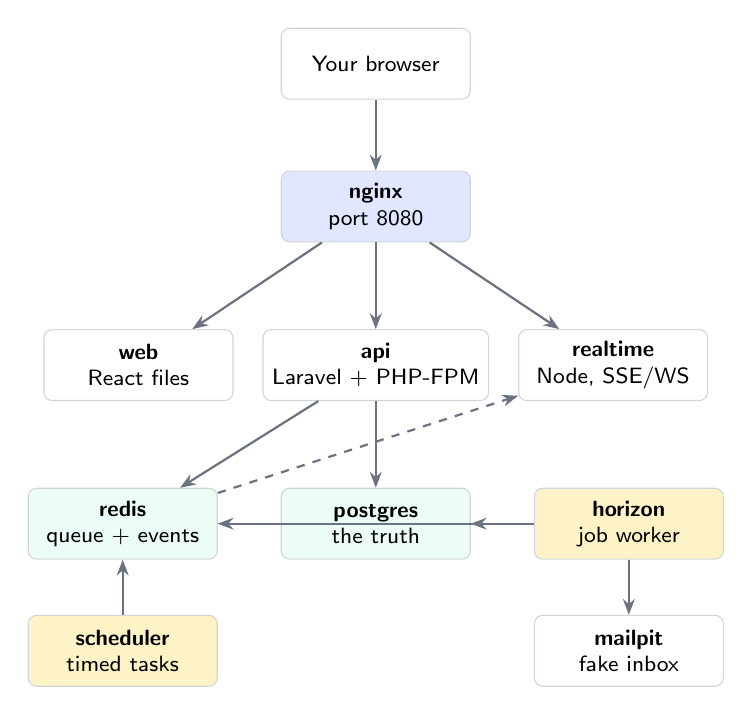
\begin{tikzpicture}[
  font=\footnotesize\sffamily,
  box/.style={draw=rule,fill=white,rounded corners=3pt,minimum height=9mm,minimum width=24mm,align=center},
  edge/.style={draw=rule,fill=brandlt,rounded corners=3pt,minimum height=9mm,minimum width=24mm,align=center},
  data/.style={draw=rule,fill=goodbg,rounded corners=3pt,minimum height=9mm,minimum width=24mm,align=center},
  work/.style={draw=rule,fill=warnbg,rounded corners=3pt,minimum height=9mm,minimum width=24mm,align=center},
  arr/.style={-{Stealth[length=2mm]},draw=muted,thick},
  evt/.style={-{Stealth[length=2mm]},draw=muted,thick,dashed},
]
\node[box] (browser) {Your browser};
\node[edge, below=9mm of browser] (nginx) {\textbf{nginx}\\port 8080};
\node[box, below left=11mm and 6mm of nginx] (web) {\textbf{web}\\React files};
\node[box, below=11mm of nginx] (api) {\textbf{api}\\Laravel + PHP-FPM};
\node[box, below right=11mm and 6mm of nginx] (rt) {\textbf{realtime}\\Node, SSE/WS};

\node[data, below=11mm of api] (pg) {\textbf{postgres}\\the truth};
\node[data, left=8mm of pg] (redis) {\textbf{redis}\\queue + events};
\node[work, right=8mm of pg] (horizon) {\textbf{horizon}\\job worker};
\node[work, below=7mm of redis] (sched) {\textbf{scheduler}\\timed tasks};
\node[box, below=7mm of horizon] (mail) {\textbf{mailpit}\\fake inbox};

\draw[arr] (browser) -- (nginx);
\draw[arr] (nginx) -- (web);
\draw[arr] (nginx) -- (api);
\draw[arr] (nginx) -- (rt);
\draw[arr] (api) -- (pg);
\draw[arr] (api) -- (redis);
\draw[evt] (redis) -- (rt);
\draw[arr] (horizon) -- (redis);
\draw[arr] (horizon) -- (pg);
\draw[arr] (sched) -- (redis);
\draw[arr] (horizon) -- (mail);
\end{tikzpicture}
\caption*{\small\color{muted}The nine containers. Solid arrows are direct
connections; the dashed arrow is events flowing from Laravel to the realtime
tier through Redis. Only nginx is reachable from outside.}
\end{figure}

\section{What each one is for}

\begin{center}
\begin{tabular}{@{}>{\raggedright\arraybackslash}p{2.4cm}>{\raggedright\arraybackslash}p{2.5cm}>{\raggedright\arraybackslash}p{9.0cm}@{}}
\toprule
\textbf{Container} & \textbf{Built from} & \textbf{Its job} \\
\midrule
\fpath{nginx} & nginx 1.27 & The front door. Everything from your browser arrives here and is routed onward. Nothing else is exposed. \\
\fpath{web} & React + Vite & Serves the compiled JavaScript and CSS. It has no logic --- it asks the API for everything. \\
\fpath{api} & PHP 8.3 + Laravel & All the rules. Who may do what, what a valid transition is, what gets written. \\
\fpath{realtime} & Node.js 22 & Holds long-lived connections open so screens update without a refresh. \\
\fpath{postgres} & PostgreSQL 16 & Stores everything. The single source of truth. \\
\fpath{redis} & Redis 7 & Two jobs: carries live events from Laravel to realtime, and holds the queue of pending work. \\
\fpath{horizon} & same as api & Runs queued jobs --- chiefly sending email --- so the web request does not wait for them. \\
\fpath{scheduler} & same as api & Runs timed tasks, like sweeping notifications that were never delivered. \\
\fpath{mailpit} & mailpit & A fake inbox for development, so test email never reaches a real person. \\
\bottomrule
\end{tabular}
\end{center}

\note{Notice that \fpath{api}, \fpath{horizon} and \fpath{scheduler} are built
from \emph{the same image}. One Dockerfile, three containers, three different
start commands. Without Docker you would install PHP once and run three
processes; here each gets its own isolated process, so a memory leak in the
queue worker cannot take the API down with it.}

\section{Following one request all the way through}

Abstract diagrams are easy to nod at and hard to remember. So follow one real
action: \textbf{a responder clicks ``Acknowledge'' on an incident.}

\begin{enumerate}[leftmargin=1.5cm]
\item The browser sends \fpath{POST /api/v1/incidents/42/status} to
  \fpath{localhost:8080}. That is \textbf{nginx}.
\item nginx sees the path starts with \fpath{/api/}, so it hands the request to
  \textbf{api} over FastCGI --- not HTTP. (FastCGI is the protocol web servers
  use to talk to PHP.)
\item Laravel checks the JWT in the \fpath{Authorization} header: who is this?
\item It checks the \emph{policy}: may a responder change this incident's
  status?
\item It checks the \emph{enum}: is \fpath{open} to \fpath{acknowledged} a legal
  move?
\item Inside one database transaction it writes the new status to
  \textbf{postgres}, appends a timeline event, and creates notification rows.
\item The transaction commits. Only then does it push jobs onto \textbf{redis}
  and publish an event.
\item \textbf{horizon} picks the job off Redis and sends email through
  \textbf{mailpit}.
\item \textbf{realtime} is subscribed to Redis. It receives the event and pushes
  it down every open connection.
\item Every other open browser updates. Nobody pressed refresh.
\end{enumerate}

\warnbox{Step 7 says ``the transaction commits, \emph{only then}'' for a
reason. If the job were queued before the commit, Horizon --- a separate process
--- could pick it up and look for an incident that has not been written yet. It
would find nothing and fail. This is one of the classic distributed-system bugs,
and the ordering in that step is the entire defence against it.}

\section{Why not one program?}

You could build all of this as a single Laravel application. Many people would.
Three things here genuinely cannot be done that way.

\begin{description}[leftmargin=1.2cm,style=nextline]
\item[Long-lived connections] PHP-FPM assigns a worker process per request. A
  connection held open for an hour would occupy a worker for an hour. Twenty
  users watching a dashboard would consume the whole pool and the API would stop
  answering anything at all. Node handles thousands of idle connections on one
  process, because that is what an event loop is good at. Hence a separate
  \fpath{realtime} service.
\item[Slow work] Sending an email takes as long as the mail server takes. If
  that happened inside the request, the responder's browser would spin while
  SMTP negotiated. So the API writes a row, returns immediately, and
  \fpath{horizon} does the sending afterwards.
\item[Timed work] Something must run every minute regardless of whether anyone
  is using the system. A web request cannot do that, because there might not be
  one. Hence \fpath{scheduler}.
\end{description}

\note{This is a \emph{modular service-oriented} architecture, not microservices.
The distinction matters: there is one database and one deployable unit. The
services are split along the lines where the \emph{runtime model} differs ---
request/response, long-lived connection, background work --- not along business
domains. Splitting by domain is what produces microservices, and with them
distributed transactions, which this system deliberately does not have.}

\section{The security boundary}

One rule, and it explains most of the configuration you will read later:
\textbf{only nginx is reachable from outside}.

\begin{center}
\begin{tabular}{@{}lll@{}}
\toprule
\textbf{Service} & \textbf{Reachable from your machine?} & \textbf{How} \\
\midrule
nginx & yes & \fpath{localhost:8080} \\
mailpit & yes (development only) & \fpath{localhost:8025} \\
postgres & development only & \fpath{localhost:5432} \\
redis & development only & \fpath{localhost:6379} \\
api & no & only nginx, over the internal network \\
realtime & no & only nginx \\
web & no & only nginx \\
horizon & no & has no network port at all \\
scheduler & no & has no network port at all \\
\bottomrule
\end{tabular}
\end{center}

In production those ``development only'' rows are closed too. You will see
exactly how in Part~III, in \fpath{docker-compose.prod.yml}.

\chapter{Every file, and why}
\label{ch:files}

You cannot hold 174 PHP files in your head, and you do not need to. What you
need is a reliable answer to one question: \emph{if I want to change X, which
folder do I open?} This chapter gives you that.

\section{The top level}

\begin{lstlisting}
D:\IncidentFlow\
|
+-- api/                  the Laravel backend  (all the rules live here)
+-- web/                  the React frontend   (what you look at)
+-- realtime/             the Node service     (live updates)
+-- infra/nginx/          the front door's configuration
+-- scripts/              operational scripts (database backup)
+-- deploy/               deployment runbooks
+-- docs/                 this book, and the screenshots in it
|
+-- docker-compose.yml        development: the nine containers
+-- docker-compose.prod.yml   production overlay (no bind mounts, no open ports)
+-- docker-compose.tls.yml    adds HTTPS for a single-server deployment
+-- Makefile                  short names for long commands
+-- README.md                 the short version of this book
\end{lstlisting}

\note{Three top-level folders --- \fpath{api}, \fpath{web}, \fpath{realtime} ---
are the three programs \emph{we} wrote. Everything else is either configuration
that wires them together or documentation. If you remember only one thing from
this chapter, remember those three.}

\section{Inside api/ --- where the rules live}

This is the largest and most important part of the system. Laravel puts almost
everything under \fpath{app/}.

\begin{center}
\begin{tabular}{@{}>{\raggedright\arraybackslash}p{4.3cm}rp{8.2cm}@{}}
\toprule
\textbf{Folder} & \textbf{Files} & \textbf{What is in it} \\
\midrule
\fpath{app/Models} & 14 & One class per database table. \fpath{Incident}, \fpath{User}, \fpath{AuditLog}. \\
\fpath{app/Http/Controllers} & 19 & The entry point for each HTTP request. \\
\fpath{app/Http/Resources} & 11 & Turns a model into the JSON the API returns. \\
\fpath{app/Http/Middleware} & 6 & Runs before a request reaches a controller. \\
\fpath{app/Http/Requests} & --- & Validates incoming data before anything touches it. \\
\fpath{app/Enums} & 9 & Fixed sets of values --- statuses, severities, roles. \\
\fpath{app/Policies} & 4 & Who is allowed to do what. \\
\fpath{app/Services} & 12 & The actual business logic, grouped by subject. \\
\fpath{app/Jobs} & 1 & Work that happens in the background. \\
\fpath{app/Console/Commands} & 3 & Things you can run by hand or on a schedule. \\
\fpath{app/Exceptions} & 6 & Named failures, and the one place errors are formatted. \\
\bottomrule
\end{tabular}
\end{center}

And outside \fpath{app/}:

\begin{center}
\begin{tabular}{@{}>{\raggedright\arraybackslash}p{4.3cm}p{9.4cm}@{}}
\toprule
\textbf{Folder} & \textbf{What is in it} \\
\midrule
\fpath{database/migrations} & 8 files that create the tables. Run in order, they build the schema from nothing. \\
\fpath{database/seeders} & Fills a fresh database with realistic demo data. \\
\fpath{routes/api.php} & The map from URL to controller. Start here when tracing anything. \\
\fpath{config/} & Settings, all reading from environment variables. \\
\fpath{tests/} & 13 test files, 114 tests. \\
\fpath{docker/} & The container's own files: entrypoint, PHP settings, nginx template. \\
\bottomrule
\end{tabular}
\end{center}

\subsection{One controller per action, not one per resource}

Open \fpath{app/Http/Controllers/Api/V1/} and you will find something unusual.

\begin{lstlisting}
AuthController.php                 IncidentSeverityController.php
AuditLogController.php             IncidentStatusController.php
HealthController.php               IncidentUpdateController.php
IncidentAssigneeController.php     MemberController.php
IncidentCommanderController.php    MetricsController.php
IncidentCommentController.php      NotificationController.php
IncidentController.php             OrganizationController.php
IncidentEventController.php        PostmortemController.php
IncidentExportController.php       RealtimeTicketController.php
                                   ServiceController.php
\end{lstlisting}

There are \emph{eight} controllers whose name begins with \fpath{Incident}. A
more common design would have one \fpath{IncidentController} with a dozen
methods on it: \fpath{updateStatus}, \fpath{changeSeverity}, \fpath{assign},
\fpath{comment}, \fpath{export}, and so on.

\note{Splitting them has a specific payoff. Changing an incident's
\emph{severity} and changing its \emph{status} need different permissions, emit
different timeline events, and notify different people. As methods on one class
they would share a file, and over time they would start sharing helper methods
and drifting into each other. As separate classes each has exactly one reason to
change, and the route file reads as a list of capabilities rather than a list of
URLs.}

\subsection{Where the real logic lives}

Controllers here are deliberately thin. They check the request, hand off, and
format the reply. The thinking happens in \fpath{app/Services}.

\begin{center}
\begin{tabular}{@{}>{\raggedright\arraybackslash}p{5.0cm}p{8.7cm}@{}}
\toprule
\textbf{Service folder} & \textbf{Responsible for} \\
\midrule
\fpath{Services/Incidents} & Creating and changing incidents; recording the timeline. Three files, and the most important code in the project. \\
\fpath{Services/Auth} & Issuing and verifying tokens, and the key pair they are signed with. \\
\fpath{Services/Notifications} & Deciding who hears about what, and writing the rows before anything is sent. \\
\fpath{Services/Realtime} & Publishing events to Redis so the realtime tier can forward them. \\
\fpath{Services/Metrics} & Computing time-to-acknowledge and time-to-resolve. \\
\fpath{Services/Audit} & Writing the append-only audit log. \\
\bottomrule
\end{tabular}
\end{center}

\warnbox{If you are ever lost in this codebase, the fastest route is:
\fpath{routes/api.php} tells you which controller handles a URL; the controller
tells you which service does the work; the service is where the answer is. Three
hops, every time. Resist the urge to grep --- following the path teaches you the
structure, and grep does not.}

\section{Inside web/ --- what you look at}

Thirty-six TypeScript files, in a conventional React layout.

\begin{center}
\begin{tabular}{@{}>{\raggedright\arraybackslash}p{4.3cm}p{9.4cm}@{}}
\toprule
\textbf{Folder} & \textbf{What is in it} \\
\midrule
\fpath{src/pages} & One file per screen. Nine of them --- and Part~II gives each its own chapter. \\
\fpath{src/components} & Pieces reused across screens: the layout, the timeline, badges, dialogs. \\
\fpath{src/lib} & The API client. Every request the browser makes goes through one file. \\
\fpath{src/auth} & Holding the signed-in user, and refreshing the token before it expires. \\
\fpath{src/hooks} & Data fetching, and the live connection to the realtime service. \\
\fpath{e2e/} & Browser tests that drive the whole stack the way a person would. \\
\fpath{docker/} & The nginx config that serves the built files. \\
\bottomrule
\end{tabular}
\end{center}

\note{\fpath{src/lib/api-client.ts} is worth finding early. \emph{Every} call
the frontend makes passes through it, which is why the token refresh, the error
shape, and the base URL are each defined exactly once. When you later read that
the API returns one consistent error envelope, this is the file that depends on
it being true.}

\section{Inside realtime/ --- the live connection}

The smallest of the three: twelve files, doing one thing --- holding connections
open and forwarding events onto them.

\begin{center}
\begin{tabular}{@{}>{\raggedright\arraybackslash}p{4.3cm}p{9.4cm}@{}}
\toprule
\textbf{File or folder} & \textbf{What it does} \\
\midrule
\fpath{src/index.ts} & Starts the server, and shuts it down carefully. \\
\fpath{src/app.ts} & The routes: \fpath{/healthz}, \fpath{/readyz}, \fpath{/stream}, \fpath{/metrics}. \\
\fpath{src/config.ts} & Reads and validates environment variables at boot. \\
\fpath{src/} (rest) & Subscribing to Redis, verifying tokens, tracking connections. \\
\bottomrule
\end{tabular}
\end{center}

\warnbox{The realtime service can \emph{verify} tokens but cannot \emph{create}
them. It is given only the public half of the signing key. This is deliberate:
the realtime tier holds thousands of open connections and is the most exposed
part of the system, so if it were ever compromised the attacker would gain the
ability to read tokens --- not to mint new ones. You will see the mechanism in
Part~II.}

\section{Everything else}

\begin{center}
\begin{tabular}{@{}>{\raggedright\arraybackslash}p{5.2cm}p{8.5cm}@{}}
\toprule
\textbf{Path} & \textbf{What it is} \\
\midrule
\fpath{infra/nginx/default.conf} & The routing table for the entire system: which URL goes to which service. Read it once and the architecture stops being abstract. \\
\fpath{infra/caddy/Caddyfile} & The HTTPS terminator, used only when deploying to a single server. \\
\fpath{scripts/backup-db.sh} & Nightly database backup. \\
\fpath{docker-compose.yml} & Defines the nine containers, their network, and their storage. \\
\fpath{Makefile} & Short aliases, so you type \fpath{make up} rather than a 90-character command. \\
\bottomrule
\end{tabular}
\end{center}

\section{A rule of thumb for finding anything}

\begin{center}
\begin{tabular}{@{}p{6.4cm}p{7.3cm}@{}}
\toprule
\textbf{You want to change\ldots} & \textbf{Open\ldots} \\
\midrule
what a screen looks like & \fpath{web/src/pages/} \\
what data a screen shows & \fpath{web/src/hooks/} \\
who is allowed to do something & \fpath{api/app/Policies/} \\
what happens when they do it & \fpath{api/app/Services/} \\
the shape of the JSON returned & \fpath{api/app/Http/Resources/} \\
a database column & \fpath{api/database/migrations/} \\
which URL reaches which code & \fpath{api/routes/api.php} \\
which service answers a URL & \fpath{infra/nginx/default.conf} \\
\bottomrule
\end{tabular}
\end{center}

\part{The guided tour}

% Part divider text: see the note in main.tex about \@endpart.
\noindent\textbf{\large What this part covers}

\medskip
\noindent
One chapter per screen. Each opens with a photograph of the running application,
then shows the code that produced it, then explains the decisions behind that
code. The file path is printed above every listing, so you can open the same
file on your own machine and read along.

\medskip
\noindent
These chapters are meant to be read at the keyboard with the stack running. If
it is not running yet, jump forward to Part~III, start it, and come back.

\chapter{Sign in}
\label{ch:login}

\shot{01-login-empty.png}{The sign-in screen. Everything an unauthenticated
visitor can see of IncidentFlow.}

\section{What is deliberately missing}

Look at the screenshot again and notice what is \emph{not} there: there are no
demo account credentials printed on the page.

They used to be. During development it is convenient to show ``sign in as
\fpath{admin@example.com} / \fpath{password}'' right on the form. It was removed,
and the reason is written into the file so nobody adds it back:

\where{web/src/pages/LoginPage.tsx}
\begin{lstlisting}[language=tsx]
/**
 * Sign-in.
 *
 * Note what is deliberately absent: demo account credentials. They used to be
 * printed here for convenience. A password rendered on a login screen trains
 * every visitor to treat this as a toy, and there is no way for a viewer to
 * tell "seeded demo password" from "real password left in the markup". They now
 * live in the README and the setup manual, where a reader has already chosen to
 * look at project documentation.
 */
\end{lstlisting}

\note{This is a small thing that says something larger. A visitor cannot tell
the difference between a password that is safe to show and one that is not ---
so showing any password teaches them that this application is careless with
them. The credentials did not disappear; they moved somewhere a reader arrives
deliberately.}

\section{The two halves of the screen}

The layout is a split panel: brand on the left, form on the right. The left half
vanishes on a narrow screen, and that is a decision rather than a default:

\where{web/src/pages/LoginPage.tsx}
\begin{lstlisting}[language=tsx]
{/* ---------------------------------------------------------------- */}
{/* Brand panel. Hidden below lg: on a phone it would push the actual */}
{/* form below the fold, which is the one thing a login page must not */}
{/* do.                                                              */}
{/* ---------------------------------------------------------------- */}
<aside className="relative hidden overflow-hidden bg-brand-900 p-12 lg:flex lg:flex-col lg:justify-between">
\end{lstlisting}

The \fpath{hidden} and \fpath{lg:flex} classes are Tailwind: hidden by default,
becoming a flex column only at the \fpath{lg} breakpoint and above. On a phone
the form is the first thing on screen.

\section{The password field, and why it has an eye}

\shot{03-login-password-revealed.png}{The reveal toggle, shown pressed. The
field's type flips between \fpath{password} and \fpath{text}.}

\where{web/src/pages/LoginPage.tsx}
\begin{lstlisting}[language=tsx]
<input
  id="password"
  type={showPassword ? 'text' : 'password'}
  autoComplete="current-password"
  required
  value={password}
  onChange={(event) => setPassword(event.target.value)}
  className="input pr-11"
/>
<button
  type="button"
  onClick={() => setShowPassword((visible) => !visible)}
  // Typos are invisible in a masked field and the error message
  // is deliberately unhelpful, so a reveal toggle is the only
  // way to tell a wrong password from a mistyped one.
  aria-label={showPassword ? 'Hide password' : 'Show password'}
  className="absolute inset-y-0 right-0 grid w-11 place-items-center ..."
>
\end{lstlisting}

Three details in that block are worth naming.

\begin{description}[leftmargin=1.2cm,style=nextline]
\item[\fpath{type=\{showPassword ? 'text' : 'password'\}}] React re-renders the
  input with a different \fpath{type} attribute. There is no separate ``visible''
  input; it is one field that changes character.
\item[\fpath{autoComplete="current-password"}] Tells the browser and password
  managers what this field is. Without it, saved passwords do not offer
  themselves, and users blame your application.
\item[\fpath{aria-label}] What a screen reader announces for a button whose
  visible content is an icon with no text.
\end{description}

\bugbox{That \fpath{aria-label} broke every end-to-end test the day it was
added. The tests located the password field with
\fpath{getByLabel('Password')}, and Playwright's \fpath{getByLabel} matches
\emph{substrings} --- so ``Password'' also matched ``Show password'' on the new
button. Two elements matched one locator, and Playwright refuses to guess. Full
story in Chapter~\ref{ch:bugs-frontend}.}

\section{What happens when you press Sign in}

\where{web/src/pages/LoginPage.tsx}
\begin{lstlisting}[language=tsx]
async function handleSubmit(event: FormEvent) {
  event.preventDefault();
  setError(null);
  setSubmitting(true);

  try {
    await login(email, password);
  } catch (cause) {
    // The server deliberately returns the same message for an unknown email
    // and a wrong password; passing it straight through keeps the client from
    // reintroducing the enumeration leak the API was careful to avoid.
    setError(
      cause instanceof ApiError ? cause.message : 'Sign-in failed. Check your connection and try again.',
    );
  } finally {
    setSubmitting(false);
  }
}
\end{lstlisting}

\fpath{event.preventDefault()} stops the browser's default behaviour of
reloading the page when a form is submitted. Without it, React never sees the
submission --- the page simply navigates.

\section{The error message is deliberately unhelpful}

\shot{02-login-error.png}{A failed sign-in. Read the message carefully.}

The message is \emph{``Those credentials do not match our records.''} It does
not say whether the email exists.

That is not laziness. Here is the server code:

\where{api/app/Http/Controllers/Api/V1/AuthController.php}
\begin{lstlisting}[language=PHP]
$user = User::query()->where('email', $credentials['email'])->first();

/**
 * Hash::check runs even when the user does not exist would be ideal for
 * constant time; Laravel's own attempt() has the same shape. The real
 * defence against enumeration here is the identical response for both
 * cases, plus the per-email+IP rate limit on this route.
 */
if ($user === null || ! Hash::check($credentials['password'], $user->password)) {
    return $this->invalidCredentials($request);
}
\end{lstlisting}

\note{This defends against \textbf{user enumeration}. If a wrong password said
``incorrect password'' and an unknown address said ``no such user'', anyone could
discover who has an account by trying addresses --- useful for phishing, and for
knowing which passwords are worth attacking. One message for both cases removes
that signal. The cost is a slightly worse experience for someone who genuinely
mistyped their address, which is why the reveal toggle exists.}

\subsection{A disabled account is treated differently}

\where{api/app/Http/Controllers/Api/V1/AuthController.php}
\begin{lstlisting}[language=PHP]
if (! $user->is_active) {
    return response()->json([
        'error' => [
            'code' => 'account_disabled',
            'message' => 'This account has been disabled. Contact an administrator.',
            'request_id' => $request->headers->get('X-Request-Id'),
        ],
    ], Response::HTTP_FORBIDDEN);
}
\end{lstlisting}

This message \emph{is} specific, and that is consistent rather than
contradictory: to reach it you must already have supplied the correct password,
so you are not an attacker probing for valid addresses --- you are the account
holder, and telling you to contact an administrator is the useful answer.

\subsection{Every error has the same shape}

Notice the JSON: \fpath{code}, \fpath{message}, \fpath{request\_id}. Every error
the API produces has that shape, from any endpoint, formatted in one place.

\where{api/app/Exceptions/ApiExceptionRenderer.php}
\begin{lstlisting}[language=PHP]
/**
 * One error shape for the entire API.
 *
 *   { "error": { "code", "message", "details", "request_id" } }
 *
 * Central error handling is not about tidiness. It is about two properties
 * that are impossible to maintain if each controller formats its own failures:
 *
 *  - the frontend has exactly one parser, and switches on a stable `code`
 *    rather than on prose that changes when someone rewords a message;
 *  - server faults never leak internals.
 */
\end{lstlisting}

The \fpath{request\_id} matters operationally: it appears in the response
\emph{and} in the server log, so a user reporting ``it failed'' can quote a
string that leads straight to the exact log line.

\section{What sign-in actually returns}

Two things, and they are stored differently on purpose.

\begin{center}
\begin{tabular}{@{}>{\raggedright\arraybackslash}p{3.3cm}>{\raggedright\arraybackslash}p{3.0cm}p{7.6cm}@{}}
\toprule
\textbf{Token} & \textbf{Lives} & \textbf{Why there} \\
\midrule
Access token & In memory (JavaScript) & Short-lived, 15 minutes. Sent on every API call. Never written to disk, so a stolen laptop does not hand it over. \\
Refresh token & \fpath{httpOnly} cookie & 30 days. JavaScript cannot read it at all, so a cross-site scripting bug cannot steal it. \\
\bottomrule
\end{tabular}
\end{center}

You can see the cookie's exact settings by signing in with \fpath{curl}:

\begin{lstlisting}[language=bash]
curl -s -i -X POST http://localhost:8080/api/v1/auth/login \
  -H 'Content-Type: application/json' \
  -d '{"email":"responder@incidentflow.test","password":"incidentflow"}' \
  | grep -i set-cookie
\end{lstlisting}

\expect{A line containing \fpath{httponly}, \fpath{samesite=lax}, and
\fpath{path=/api/v1/auth}. That path is a deliberate narrowing: the cookie is
only ever sent to the four authentication endpoints, so it is not attached to
the hundreds of other API calls that have no use for it.}

\warnbox{In production the same cookie also carries \fpath{Secure}, which means
the browser will only send it over HTTPS. This has a consequence that has caught
many people, including during this project: deploy over plain HTTP and sign-in
\emph{appears} to work, then the session dies about fifteen minutes later when
the access token expires and the refresh cookie is never sent back. Nothing
errors, and no log records it. Chapter~\ref{ch:bugs-deploy} covers it.}

\section{Check your understanding}

\begin{itemize}[leftmargin=1.4cm]
\cbox Why does the sign-in error not tell you whether the email exists?
\cbox Why is the access token kept in memory rather than \fpath{localStorage}?
\cbox Why can JavaScript not read the refresh cookie?
\cbox What would break if \fpath{event.preventDefault()} were removed from
  \fpath{handleSubmit}?
\end{itemize}

\chapter{The incidents list}
\label{ch:incidents}

\shot{05-incidents-list.png}{The incidents list, signed in as an incident
commander. This is the screen people leave open all day.}

\section{Reading the screen}

Seven columns, and each answers a question an on-call engineer actually asks.

\begin{center}
\begin{tabular}{@{}>{\raggedright\arraybackslash}p{4.4cm}p{9.3cm}@{}}
\toprule
\textbf{Column} & \textbf{The question it answers} \\
\midrule
Reference & ``Which incident are we talking about?'' A short stable code you can say out loud on a call. \\
Severity & ``How bad?'' \\
Status & ``Is anyone on it?'' \\
Title & ``What is it?'' \\
Service & ``What is affected?'' \\
Opened & ``When did this start?'' \\
Running / resolved in & ``How long has this been going on --- or how long did it take?'' \\
\bottomrule
\end{tabular}
\end{center}

\note{That last column changes meaning depending on the row. For a live incident
it counts up; for a finished one it is a fixed duration. One column, two
meanings, and it works because you always want the same thing: elapsed time that
matters right now.}

\section{The button that is not always there}

\where{web/src/pages/IncidentsPage.tsx}
\begin{lstlisting}[language=tsx]
{can('incident.create') && (
  <button
    type="button"
    onClick={() => setCreating(true)}
    className="btn btn-primary"
  >
    <Plus className="h-4 w-4" aria-hidden="true" />
    Report incident
  </button>
)}
\end{lstlisting}

That \fpath{\&\&} is JavaScript's short-circuit: if \fpath{can('incident.create')}
is false, the expression evaluates to false and React renders nothing. The
button does not appear disabled --- it does not exist.

Compare the same screen seen by a viewer:

\shot{11-incidents-as-viewer.png}{The identical page, signed in as Sofia Rossi,
a viewer. The ``Report incident'' button is gone. So is ``Export CSV''.}

\warnbox{This is presentation only. A viewer who opens the browser console and
sends \fpath{POST /api/v1/incidents} directly is not stopped by a missing
button, because the button was never the control. The API refuses the request
using a policy on the server. Hiding it is politeness --- it keeps people from
attempting things they cannot do. Chapter~\ref{ch:roles} shows both halves side
by side.}

\section{Where \fpath{can()} comes from}

The frontend is told, at sign-in, exactly what this user may do. It does not
guess from the role name --- it receives a list of permission strings and checks
membership. That matters: the mapping from role to permissions lives in the API,
in one place, and the frontend never has a second copy of it that could drift.

\section{Every badge is an enum}

\where{web/src/pages/IncidentsPage.tsx}
\begin{lstlisting}[language=tsx]
<td className="px-3 py-2">
  <SeverityBadge severity={incident.severity.value} label={incident.severity.label} />
</td>
<td className="px-3 py-2">
  <StatusBadge status={incident.status.value} label={incident.status.label} />
</td>
\end{lstlisting}

Notice the API sends \emph{both} \fpath{value} and \fpath{label}: the machine
form (\fpath{sev1}) and the human form (\fpath{Critical}). The badge colours
itself from \fpath{value} and prints \fpath{label}.

\note{The alternative --- sending only \fpath{sev1} and having the frontend hold
a lookup table of display names --- means two copies of the same knowledge. Add
a severity level and you must remember to update the other side. Sending both
means the API stays the single source of truth for what its own values mean.}

\section{The colour rule this whole design follows}

\where{web/src/index.css}
\begin{lstlisting}
/* red means severity ... So the brand itself is deliberately not red. */
\end{lstlisting}

In an incident tool, red already has a job: it means \emph{this is bad}. If the
brand colour were also red, every page would be permanently alarming and a real
\fpath{sev1} would not stand out. So the brand is indigo, and red is reserved
for severity alone.

That single rule explains the entire palette --- and it is the sort of decision
that is obvious in hindsight and invisible unless someone writes it down.

\section{Filtering, and why the URL changes}

The filter bar above the table --- search, severity, status, service --- writes
its state into the page's URL. That is why you can copy the address of
``all open sev1 incidents on the payments service'' and send it to a colleague,
and why the browser Back button steps through your filters.

\note{Storing view state in the URL rather than in a variable is a small amount
of extra work that turns a screen into something shareable. On an incident call,
pasting a link is faster than describing which dropdowns to set.}

\section{Check your understanding}

\begin{itemize}[leftmargin=1.4cm]
\cbox Why does the API send both \fpath{value} and \fpath{label} for a severity?
\cbox A viewer cannot see ``Report incident''. What actually stops them creating
  an incident?
\cbox Why is the brand colour not red?
\cbox What is gained by putting filter state in the URL?
\end{itemize}

\chapter{The incident detail page and its timeline}
\label{ch:detail}

\shot{06-incident-detail.png}{One incident, open. The timeline runs down the
page; the controls for changing it sit alongside.}

This is the most important screen in the application. Everything else exists to
get you here or to summarise what happened here.

\section{The timeline is the product}

Everything that has ever happened to this incident appears as an entry: it was
opened, someone acknowledged it, severity was raised, a note was posted, it was
mitigated, it was resolved.

\where{web/src/components/Timeline.tsx}
\begin{lstlisting}[language=tsx]
{events.map((event) => {
  const { relative, absolute } = formatTimestamp(event.occurred_at);
  return (
    <li key={event.id} className="relative">
      <span className={dotColour(event.type)} />
      <p className="text-sm text-slate-800 dark:text-slate-200">{event.summary}</p>
      <time dateTime={event.occurred_at ?? undefined}>{relative}</time>
      {typeof event.payload.note === 'string' && event.payload.note.length > 0 && (
        <p>{event.payload.note}</p>
      )}
      {event.request_id && (
        <span>{event.request_id}</span>
      )}
    </li>
  );
})}
\end{lstlisting}

Two details repay attention.

\begin{description}[leftmargin=1.2cm,style=nextline]
\item[Both time formats] \fpath{relative} shows ``12 minutes ago'', which is what
  you want during an incident. \fpath{dateTime} carries the exact machine
  timestamp, which is what you want when writing the postmortem. The
  \fpath{<time>} element is the HTML built for exactly this.
\item[\fpath{request\_id} on the entry] Every timeline event records the ID of
  the HTTP request that created it. When something looks wrong six months later,
  that string leads to the precise server log line. Very few systems do this,
  and it costs one column.
\end{description}

\section{Append-only, enforced three times}

Chapter~\ref{ch:arch} claimed the timeline cannot be edited. Here is the
enforcement.

\where{api/app/Models/IncidentEvent.php}
\begin{lstlisting}[language=PHP]
/**
 * Corrections are appended as new events, never applied in place.
 */
protected static function booted(): void
{
    static::updating(static function (): never {
        throw new LogicException('Incident timeline events are append-only and cannot be modified.');
    });

    static::deleting(static function (): never {
        throw new LogicException('Incident timeline events are append-only and cannot be deleted.');
    });
}
\end{lstlisting}

\fpath{booted()} runs once when the class is first used, and registers two
listeners. Any attempt to save a change to an existing event, or to delete one,
throws --- from anywhere in the codebase, including a future controller written
by someone who never read this book.

\note{The return type \fpath{: never} is doing real work. It tells PHP --- and
any static analyser --- that this function cannot return normally; it always
throws. A reader skimming the file learns the guarantee from the signature
without reading the body.}

\subsection{Why three layers and not one}

\begin{center}
\begin{tabular}{@{}>{\raggedright\arraybackslash}p{3.0cm}>{\raggedright\arraybackslash}p{4.4cm}p{6.4cm}@{}}
\toprule
\textbf{Layer} & \textbf{What it stops} & \textbf{What it cannot stop} \\
\midrule
API & Requests that ask to edit history --- there is no such endpoint. & Code inside the application calling the model directly. \\
Model & Any PHP code in this project, deliberate or accidental. & Someone connecting to PostgreSQL and running \fpath{UPDATE}. \\
Schema & Structure: there is no ``edited\_at'', no soft-delete column, nowhere for a revision to live. & A determined administrator with database credentials. \\
\bottomrule
\end{tabular}
\end{center}

\warnbox{No layer is complete on its own, and the last row is honest: a person
with direct database access can change anything. The guarantee is not
mathematical --- it is that no \emph{ordinary} path through the system can
rewrite history, and that doing so requires deliberate, logged, out-of-band
action rather than a stray line of application code.}

\section{Changing an incident}

The controls beside the timeline are gated by permission, the same way the
``Report incident'' button was in Chapter~\ref{ch:incidents}. But status changes
carry a second gate the list page did not have: even a user \emph{with}
permission may only make a \emph{legal} move.

Recall the transition table from Chapter~\ref{ch:arch}: an incident that is
\fpath{open} may become \fpath{acknowledged} or \fpath{resolved} --- and nothing
else. The frontend shows only those two options. The API independently checks
the same rule and returns \fpath{409 Conflict} for anything else.

\note{Two independent checks of one rule sounds redundant, and it is --- on
purpose. They fail differently. The frontend check fails \emph{invisibly}: the
option is not offered, so the mistake is never made. The API check fails
\emph{loudly}: a 409 with a message. One is for people, the other is for
programs, and only the second is a security control.}

\section{The page updates while you watch it}

Open this incident in two browsers, change the status in one, and the other
updates within a second --- no refresh.

That is the \fpath{realtime} container. The chain, end to end:

\begin{enumerate}[leftmargin=1.5cm]
\item The API commits the change to PostgreSQL.
\item After the commit, it publishes a small event to Redis.
\item \fpath{realtime} is subscribed to Redis and receives it.
\item It writes the event down every open connection belonging to that
  organisation.
\item Each browser receives it and updates the page in place.
\end{enumerate}

\warnbox{Step 4 says ``belonging to that organisation'' and that phrase is
load-bearing. Every connection is authenticated, and events are filtered by
organisation before being written. Without that filter, a live stream is a
spectacular data leak: every customer would receive every other customer's
incidents in real time, and no page in the UI would ever reveal it.}

\subsection{Why the browser cannot just use its normal token}

The realtime connection is opened by the browser's \fpath{EventSource}, which
cannot set an \fpath{Authorization} header. So the frontend first asks the API
for a short-lived \emph{ticket}, then opens the stream with that ticket in the
query string.

\note{A ticket is used rather than the access token because query strings are
not private: they appear in server logs, proxy logs and browser history. A
ticket is valid for seconds, for one connection, and grants nothing but the
right to listen. Leaking it in a log is uninteresting; leaking your access token
there is not.}

\section{Check your understanding}

\begin{itemize}[leftmargin=1.4cm]
\cbox Name the three layers that stop the timeline being edited, and what each
  one misses.
\cbox Why is the same transition rule checked in both the browser and the API?
\cbox Why does a timeline entry store a \fpath{request\_id}?
\cbox Why does the live stream use a ticket instead of the access token?
\end{itemize}

\chapter{Services, metrics and postmortems}
\label{ch:screens}

Three shorter screens. Each exists because a different person asks a different
question after --- or before --- an incident.

\section{Services: what can break}

\shot{07-services.png}{The services registry. Every incident is attached to one
of these.}

A \emph{service} is a named part of your system: the payments API, the search
cluster, the mobile gateway. Incidents attach to one.

\note{This is why the incidents list can be filtered by service, and why the
metrics page can say ``the payments API had four incidents this month''. Without
a registry you would have a free-text field, everyone would spell things
differently, and no grouping would ever be reliable. A dropdown of known values
is a small constraint that makes every downstream question answerable.}

Each service carries an owning team and a criticality. Only an administrator can
add or change one --- the registry is reference data, and reference data that
anyone can edit stops being reference data.

\section{Metrics: are we getting better or worse?}

\shot{08-metrics.png}{Reliability metrics over a chosen window.}

Two numbers dominate this page, and both are industry standard.

\begin{center}
\begin{tabular}{@{}>{\raggedright\arraybackslash}p{2.2cm}>{\raggedright\arraybackslash}p{4.4cm}p{7.2cm}@{}}
\toprule
\textbf{Metric} & \textbf{Full name} & \textbf{What it tells you} \\
\midrule
MTTA & Mean time to acknowledge & How long before a human picks it up. Measures your \emph{alerting and staffing}. \\
MTTR & Mean time to resolve & How long from report to fixed. Measures your \emph{systems and tooling}. \\
\bottomrule
\end{tabular}
\end{center}

\note{The distinction matters when deciding what to fix. A bad MTTA and a good
MTTR means alerts are not reaching people --- a rota problem. A good MTTA and a
bad MTTR means people respond promptly and then struggle --- a tooling or
architecture problem. One number cannot tell you which, which is why there are
two.}

\subsection{The numbers are precomputed, not counted on the fly}

\where{api/app/Services/Metrics/}
\begin{lstlisting}[language=PHP]
/**
 * Reliability metrics: MTTA, MTTR, throughput and acknowledgement-SLA
 * ...
 * columns `time_to_acknowledge_seconds` and `time_to_resolve_seconds` are
 * ...
 * `percentile_cont` nor `date_trunc` exists in SQLite, and a metrics endpoint
 */
\end{lstlisting}

When an incident is acknowledged, the elapsed seconds are written onto the
incident row there and then. The metrics page averages a stored number rather
than recomputing durations by scanning the timeline.

\note{Storing a derived value is normally poor practice --- it can drift from
the truth. It is right here because the value is \emph{immutable once written}:
the moment of acknowledgement never changes, so the duration never changes
either. The rule of thumb is that caching a derived value is safe exactly when
its inputs can no longer move.}

\warnbox{That comment mentions SQLite, and it is a warning from experience. The
tests run on SQLite for speed; production runs PostgreSQL.
\fpath{percentile\_cont} and \fpath{date\_trunc} exist only in the latter. Code
written naturally against PostgreSQL passes review, fails in the test suite, and
--- worse --- code written to satisfy SQLite can behave differently in
production. Chapter~\ref{ch:bugs-backend} contains a bug of exactly this
family.}

\section{Postmortems: what did we learn?}

\shot{09-postmortems.png}{Postmortems --- the written record produced after an
incident is closed.}

A postmortem is the document written afterwards: what happened, why, what was
done, and what will change so it does not recur.

\subsection{Postmortems are editable --- and that is not a contradiction}

The timeline cannot be edited. A postmortem can. That is deliberate and worth
being precise about.

\begin{center}
\begin{tabular}{@{}>{\raggedright\arraybackslash}p{3.4cm}>{\raggedright\arraybackslash}p{4.2cm}p{6.2cm}@{}}
\toprule
& \textbf{Timeline} & \textbf{Postmortem} \\
\midrule
What it records & What happened & What we understood \\
Can change? & Never & Yes, until published \\
Why & Facts do not change & Understanding improves \\
\bottomrule
\end{tabular}
\end{center}

\where{api/app/Models/Postmortem.php}
\begin{lstlisting}[language=PHP]
public function isPublished(): bool
{
    return $this->status === PostmortemStatus::Published;
}
\end{lstlisting}

A postmortem is a \emph{draft} while being written, and \emph{published} when
finished. Publishing is the point at which it stops being a working document.

\note{This is the same distinction a newspaper makes between a reporter's notes
and a printed article. Conflating them --- letting people quietly revise the
record of events because their understanding changed --- is exactly the failure
mode the append-only timeline exists to prevent.}

\section{Two screens you will meet by accident}

\subsection{Registering an organisation}

\shot{04-register.png}{Creating an organisation. The first account becomes its
owner.}

There is no ``create an account'' for an existing organisation on this screen ---
registering creates an \emph{organisation} and makes you its administrator.
Everyone else is invited from inside.

\warnbox{This is why a production deployment has no demo logins. The seeder
refuses to run outside development, so on a fresh production database the very
first thing you do is register, and that first registration becomes the owner.
Part~III walks through it.}

\subsection{The page that is not there}

\shot{10-not-found.png}{An unknown URL, inside the application shell.}

Notice the navigation is still present. The 404 is rendered \emph{inside} the
layout, so a mistyped link leaves you somewhere you can navigate away from,
rather than at a dead end.

\note{A single-page application has to be told to do this. The server does not
know which paths are real --- it hands \fpath{index.html} to every unknown URL
and lets the router decide. That is the \fpath{try\_files \$uri \$uri/
/index.html} line in the web container's nginx config, and without it a hard
refresh on \fpath{/incidents/42} would return a genuine 404 while clicking
through to the same page worked fine.}

\section{Check your understanding}

\begin{itemize}[leftmargin=1.4cm]
\cbox Why is a service registry better than a free-text field?
\cbox What does a good MTTA with a bad MTTR suggest you should fix?
\cbox Why is it acceptable to store \fpath{time\_to\_resolve\_seconds} on the
  incident row?
\cbox Why may a postmortem be edited when the timeline may not?
\end{itemize}

\chapter{Permissions, seen rather than described}
\label{ch:roles}

Permission systems are usually taught as a grid, and the grid is forgettable.
This chapter teaches it differently: the same page, photographed three times,
signed in as three different people.

\section{One page, three people}

\shot{11-incidents-as-viewer.png}{\textbf{Sofia Rossi --- viewer.} She can read
everything and change nothing. No ``Report incident''. No ``Export CSV''.}

\shot{05-incidents-list.png}{\textbf{Daniel Okoye --- incident commander.} The
same data, plus the ability to act on it.}

\shot{12-incidents-as-admin.png}{\textbf{Riya Sharma --- administrator.} As the
commander, plus organisation-level control and an ``Admin'' item in the
navigation.}

Nothing about the data changed between those three pictures. What changed is
what is \emph{offered}.

\section{Where the difference is defined}

Exactly one file, and it is short enough to read in full.

\where{api/app/Enums/OrganizationRole.php}
\begin{lstlisting}[language=PHP]
public function permissions(): array
{
    $viewer = [
        Permission::IncidentView,
        Permission::PostmortemView,
        Permission::ServiceView,
        Permission::MemberView,
        Permission::MetricsView,
    ];

    $reporter = [
        ...$viewer,
        Permission::IncidentCreate,
        Permission::CommentCreate,
    ];

    $responder = [
        ...$reporter,
        Permission::IncidentUpdate,
        Permission::IncidentTransition,
        Permission::UpdateCreate,
    ];

    $commander = [
        ...$responder,
        Permission::IncidentAssign,
        Permission::IncidentCommand,
        Permission::CommentModerate,
        Permission::PostmortemManage,
        Permission::PostmortemPublish,
        Permission::ExportRun,
    ];

    return match ($this) {
        self::Viewer            => $viewer,
        self::Reporter          => $reporter,
        self::Responder         => $responder,
        self::IncidentCommander => $commander,
        self::Administrator     => [
            ...$commander,
            Permission::IncidentDelete,
            Permission::ServiceManage,
            Permission::MemberManage,
            Permission::AuditView,
            Permission::OrganizationManage,
        ],
    };
}
\end{lstlisting}

\subsection{Read the shape, not just the contents}

The \fpath{...} is PHP's spread operator: \fpath{...\$viewer} means ``everything
a viewer can do, and then these as well''. Each role is literally written as the
previous one plus a few additions.

\note{This makes the hierarchy \emph{structural} rather than a convention
somebody has to maintain. It is impossible to give a reporter a permission a
viewer lacks by accident, because a reporter's list is built from the viewer's.
A flat table --- five arrays written out in full --- would allow that mistake,
and would allow the five lists to drift apart over years of small edits.}

\subsection{Permissions are an enum, not strings}

\fpath{Permission::IncidentCreate}, not \fpath{'incident.create'}. Typing
\fpath{Permission::IncidentCreat} is an error your editor catches before you
save; typing \fpath{'incident.creat'} is a permission check that silently returns
false forever --- and a silently-false permission check fails \emph{open} or
\emph{closed} depending on which side of the comparison it lands, neither of
which you will notice in testing.

\section{Now the same picture from the other side}

The screenshots showed the frontend. Here is what actually enforces it:

\where{api/app/Enums/OrganizationRole.php}
\begin{lstlisting}[language=PHP]
public function has(Permission $permission): bool
{
    return in_array($permission, $this->permissions(), strict: true);
}
\end{lstlisting}

\fpath{strict: true} compares type as well as value. Without it PHP's loose
comparison can produce surprising equalities, and a permission check is the last
place you want a surprise.

\warnbox{Say this to yourself until it is automatic: \textbf{the missing button
is not the security}. A viewer who opens the browser console and sends the
request by hand meets this check on the server, and is refused with 403. If you
ever find yourself relying on a hidden control to prevent something, you have
not prevented it.}

\section{The full grid, for reference}

\begin{center}
\begin{tabular}{@{}>{\raggedright\arraybackslash}p{5.2cm}ccccc@{}}
\toprule
\textbf{Can\ldots} & \rotatebox{60}{viewer} & \rotatebox{60}{reporter} & \rotatebox{60}{responder} & \rotatebox{60}{commander} & \rotatebox{60}{admin} \\
\midrule
view incidents, services, metrics & yes & yes & yes & yes & yes \\
create an incident & --- & yes & yes & yes & yes \\
comment & --- & yes & yes & yes & yes \\
change status & --- & --- & yes & yes & yes \\
post an update & --- & --- & yes & yes & yes \\
assign people & --- & --- & --- & yes & yes \\
change severity & --- & --- & --- & yes & yes \\
publish a postmortem & --- & --- & --- & yes & yes \\
export CSV & --- & --- & --- & yes & yes \\
manage services & --- & --- & --- & --- & yes \\
manage members & --- & --- & --- & --- & yes \\
read the audit log & --- & --- & --- & --- & yes \\
\bottomrule
\end{tabular}
\end{center}

\section{Try it yourself}

With the stack running, sign in as each of these in turn. The password for every
demo account is \fpath{incidentflow}.

\begin{itemize}[leftmargin=1.4cm]
\cbox \fpath{viewer@incidentflow.test} --- confirm ``Report incident'' is absent.
\cbox \fpath{reporter@incidentflow.test} --- it appears. Open an incident and
  confirm you cannot change its status.
\cbox \fpath{responder@incidentflow.test} --- now you can.
\cbox \fpath{commander@incidentflow.test} --- assignment and severity appear.
\cbox \fpath{admin@incidentflow.test} --- an ``Admin'' item appears in the
  navigation.
\end{itemize}

\expect{Five sign-ins, five visibly different versions of the same application.
If two of them look identical, you are still signed in as the previous user ---
sign out properly between them.}

\chapter{The operator surfaces}
\label{ch:operator}

Three screens that users never see. They are for whoever runs the system --- and
during development, that is you.

\section{Admin: the audit log}

\shot{13-admin.png}{The administration screen. Members, services, and the audit
log.}

The audit log is the part worth studying. Every action that changes anything is
recorded here: who did it, to what, and when.

\note{This is a \emph{second} append-only record, and it is not the same thing
as the incident timeline. The timeline answers ``what happened to this
incident?'' and is visible to everyone. The audit log answers ``what did this
\emph{person} do?'' across the whole organisation, and only an administrator can
read it. One is the story of an event; the other is the story of an actor.}

You saw it being written during sign-in, in Chapter~\ref{ch:login}:

\where{api/app/Http/Controllers/Api/V1/AuthController.php}
\begin{lstlisting}[language=PHP]
$this->audit->record('auth.logged_in', $user, $user);
\end{lstlisting}

Three arguments: what happened, who did it, and what it happened to. For a
sign-in the actor and the subject are the same person, which is why \fpath{\$user}
appears twice.

\section{Horizon: watching the queue}

\shot{14-horizon-dashboard.png}{Laravel Horizon at
\fpath{http://localhost:8080/horizon}. Jobs processed, jobs failed, throughput.}

Chapter~\ref{ch:arch} said the API writes a notification row and returns
immediately, leaving \fpath{horizon} to do the sending. This is where you watch
that happen.

It answers questions that are otherwise invisible:

\begin{itemize}[leftmargin=1.4cm]
\item Are jobs being processed at all, or is the queue silently stuck?
\item Is anything failing repeatedly?
\item How long is work waiting before it is picked up?
\end{itemize}

\warnbox{This dashboard was completely broken for most of this project's life,
and nothing detected it. The page returned HTTP 200. The server logs were clean.
The health checks passed. It simply rendered a blank dark rectangle, and the
only evidence anywhere was in the browser's developer console.
Chapter~\ref{ch:bugs-infra} is that investigation in full --- it is the single
best example in this book of a failure that no amount of reading the server logs
would ever have found.}

\section{Mailpit: catching email that must not escape}

\shot{15-mailpit.png}{Mailpit at \fpath{http://localhost:8025}. Every email the
system has sent, and not one of them delivered to a real person.}

In development, IncidentFlow sends its email to \fpath{mailpit} instead of a
real mail server. Mailpit accepts everything and delivers nothing, showing it in
a web inbox instead.

\note{This is not merely convenient. The seeded database contains addresses like
\fpath{commander@incidentflow.test}, but a realistic test dataset eventually
contains something that looks like a real address --- and a \fpath{sev1}
notification mails every responder in the organisation. Without a catcher,
running the test suite once could send mail to strangers. Mailpit makes that
mistake impossible rather than unlikely.}

\subsection{Watch the whole chain in one action}

This is the best single exercise in the book, because it exercises five
containers at once.

\begin{enumerate}[leftmargin=1.5cm]
\item Open \fpath{http://localhost:8025} in one tab. It should be empty or
  nearly so.
\item In another tab, sign in as \fpath{commander@incidentflow.test} and create
  an incident with severity \textbf{sev1}.
\item Watch the Mailpit tab.
\end{enumerate}

\expect{Email appears in Mailpit within a second or two, one per responder in
the organisation. You have just watched: the \textbf{api} write rows and commit;
\textbf{redis} carry the job; \textbf{horizon} pick it up; \textbf{mailpit}
receive the result --- and \textbf{postgres} holding the record throughout.}

\warnbox{If no mail arrives, the fault is almost always Horizon rather than the
mail path. Check \fpath{docker compose logs horizon}, and check the Horizon
dashboard for failed jobs. A notification row that stays \fpath{pending} means
the job was never queued or never ran; one marked \fpath{failed} means it ran
and threw.}

\subsection{Try the same thing at sev3}

Create a second incident, this time \textbf{sev3}. No email arrives.

That is the rule from Chapter~\ref{ch:what}: only \fpath{sev1} and \fpath{sev2}
notify the whole responder pool. You have now seen one enum value decide whether
a hundred people are interrupted --- which is the concrete reason changing
severity is a permission most roles do not have.

\section{Check your understanding}

\begin{itemize}[leftmargin=1.4cm]
\cbox What question does the audit log answer that the incident timeline does
  not?
\cbox Why does sending email through a queue make the API faster \emph{and}
  more reliable?
\cbox Why is a mail catcher a safety feature rather than a convenience?
\cbox A notification row is stuck at \fpath{pending}. What are the two
  possibilities?
\end{itemize}

\part{Running it}

\noindent\textbf{\large What this part covers}

\medskip
\noindent
Everything needed to take this project from a folder on disk to a working
application, assuming you know how to open a folder in VS Code and nothing more.
Every command is given in full, with what it does, where you must be standing
when you type it, and what you should see afterwards.

\medskip
\noindent
It also answers the question people are usually too embarrassed to ask: how many
separate things are running, and how do they find each other?

\chapter{From nothing to running}
\label{ch:running}

\section{What you need installed}

Exactly one thing.

\begin{center}
\begin{tabular}{@{}>{\raggedright\arraybackslash}p{4.0cm}p{9.6cm}@{}}
\toprule
\textbf{Tool} & \textbf{Why} \\
\midrule
Docker Desktop & Runs all nine containers. Includes \fpath{docker compose}. \\
Git & To obtain the code. \\
\bottomrule
\end{tabular}
\end{center}

\note{You do \textbf{not} need PHP, Node.js, PostgreSQL or Redis installed. That
is the entire point of Docker, and it is worth pausing on: installing PHP 8.3
with the \fpath{pdo\_pgsql} extension compiled against PostgreSQL headers is
genuinely unpleasant on Windows. Docker does it once, inside an image, on every
machine identically.}

\section{The three commands that start everything}

Open a terminal. On Windows, press Start, type \fpath{powershell}, press Enter.

\begin{lstlisting}[language=bash]
cd D:\IncidentFlow
docker compose up -d --build
\end{lstlisting}

\begin{description}[leftmargin=1.4cm,style=nextline]
\item[\fpath{up}] create and start the containers
\item[\fpath{-d}] detached --- run in the background and give the prompt back
\item[\fpath{--build}] build the images from source first, rather than reusing
  whatever was built last
\end{description}

The first run takes several minutes: it downloads base images and compiles PHP
extensions. Later runs take seconds.

\begin{lstlisting}[language=bash]
docker compose ps
\end{lstlisting}

\expect{Nine rows. \fpath{postgres}, \fpath{redis}, \fpath{mailpit},
\fpath{api}, \fpath{realtime}, \fpath{web}, \fpath{nginx} should say
\fpath{healthy}. \fpath{horizon} and \fpath{scheduler} say only \fpath{Up} ---
they have no HTTP port to check, which is correct and not a fault.}

Then load the database:

\begin{lstlisting}[language=bash]
docker compose run --rm migrate
\end{lstlisting}

\expect{A list of migrations, each ending \fpath{DONE}, then seeding output
ending with \emph{``Demo accounts seeded. Password for all of them:
incidentflow''}.}

Now open \fpath{http://localhost:8080}.

\warnbox{If you see the page but signing in fails, the API is not reachable
through nginx even though both containers are ``up''. Run \fpath{curl
http://localhost:8080/api/v1/health/ready}. A \fpath{502} means nginx cannot
reach the API --- see Chapter~\ref{ch:bugs-infra}, where exactly this happened
and the cause was not what it appeared to be.}

\section{Shorter names for the same commands}

\fpath{Makefile} at the project root defines aliases. \fpath{make up} is
\fpath{docker compose up --build}, and so on.

\begin{center}
\begin{tabular}{@{}>{\raggedright\arraybackslash}p{3.2cm}p{10.4cm}@{}}
\toprule
\textbf{Command} & \textbf{What it does} \\
\midrule
\fpath{make up} & Build and start the whole stack. \\
\fpath{make down} & Stop everything \textbf{and remove the volumes}. \\
\fpath{make logs} & Follow every service's output. \\
\fpath{make shell} & Open a shell inside the API container. \\
\fpath{make migrate} & Apply pending migrations. \\
\fpath{make seed} & Load the demo organisation and 90 days of history. \\
\fpath{make fresh} & Drop everything and rebuild the schema with demo data. \\
\fpath{make test} & Run all three test suites. \\
\fpath{make lint} & Formatting and static checks across all three projects. \\
\fpath{make keys} & Generate a new RS256 key pair. \\
\bottomrule
\end{tabular}
\end{center}

\warnbox{\fpath{make down} removes the volumes. That deletes the database ---
every incident, every timeline entry, every user. It is the right behaviour for
a development alias you use to get back to a clean state, and it is a disaster
if you type it on a server. Chapter~\ref{ch:bugs-infra} includes the day this
distinction stopped being theoretical.}

\warnbox{\fpath{make keys} signs every user out immediately, everywhere. The
tokens they hold were signed with the old key and will no longer verify. That is
correct --- it is how you respond to a leaked key --- but it is not something to
run casually.}

\section{Which command runs where}

This trips up nearly everyone at first. There are three different places a
command can be typed, and typing one in the wrong place produces confusing
errors.

\begin{center}
\begin{tabular}{@{}>{\raggedright\arraybackslash}p{4.6cm}>{\raggedright\arraybackslash}p{4.0cm}p{5.0cm}@{}}
\toprule
\textbf{Command starts with} & \textbf{Runs} & \textbf{From where} \\
\midrule
\fpath{docker compose ...} & on your machine & \fpath{D:\textbackslash IncidentFlow} \\
\fpath{docker compose exec api ...} & inside the API container & anywhere in the project \\
\fpath{npm ...} & on your machine & \fpath{web/} or \fpath{realtime/} \\
\fpath{php artisan ...} & inside the API container & prefix it with \fpath{docker compose exec api} \\
\bottomrule
\end{tabular}
\end{center}

\note{\fpath{php artisan} is the one that catches people. Typing it directly in
PowerShell fails, because PHP is not installed on your machine --- it is inside
the container. Every \fpath{artisan} command in this book is written with its
\fpath{docker compose exec api} prefix for that reason.}

\section{How the nine containers find each other}

Inside Docker, \textbf{the service name is the hostname}. When the API connects
to the database it uses the host \fpath{postgres} --- not an IP address, not
\fpath{localhost}.

\where{docker-compose.yml}
\begin{lstlisting}[language=yamlx]
DB_HOST: postgres
REDIS_HOST: redis
\end{lstlisting}

Docker runs a small DNS server on the container network; \fpath{postgres}
resolves to whatever address that container currently has.

\warnbox{``Whatever address it currently has'' is the important half. Restart a
container and it may get a different one. Anything that resolved the old address
and cached it is now talking to nothing --- which is precisely how this project's
nginx started returning 502 while every container reported healthy.
Chapter~\ref{ch:bugs-infra}.}

\subsection{The complete connection map}

\begin{center}
\begin{tabular}{@{}>{\raggedright\arraybackslash}p{2.6cm}>{\raggedright\arraybackslash}p{3.0cm}>{\raggedright\arraybackslash}p{2.0cm}p{5.6cm}@{}}
\toprule
\textbf{From} & \textbf{To} & \textbf{Port} & \textbf{Carrying} \\
\midrule
your browser & nginx & 8080 & everything \\
nginx & web & 80 & the React files \\
nginx & api & 9000 & FastCGI (not HTTP) \\
nginx & realtime & 3001 & the live stream \\
api & postgres & 5432 & SQL \\
api & redis & 6379 & jobs and events \\
horizon & redis & 6379 & taking jobs off the queue \\
horizon & postgres & 5432 & reading what to send \\
horizon & mailpit & 1025 & SMTP \\
scheduler & redis & 6379 & queueing timed work \\
realtime & redis & 6379 & subscribing to events \\
\bottomrule
\end{tabular}
\end{center}

\note{Only the first row crosses the boundary of your machine. Everything else
happens on a private network Docker creates, which is why \fpath{api} has no
published port and cannot be reached from your browser at all.}

\section{Watching it work}

\begin{lstlisting}[language=bash]
docker compose logs -f api
docker compose logs -f horizon
docker compose logs --tail 50 nginx
\end{lstlisting}

\fpath{-f} follows --- new lines appear as they happen. Press Ctrl+C to stop
watching; that stops the \emph{watching}, not the container.

\subsection{Getting inside a container}

\begin{lstlisting}[language=bash]
docker compose exec api sh
\end{lstlisting}

You are now in a shell inside the API container. \fpath{php artisan} works here
without a prefix, because this is where PHP lives. Type \fpath{exit} to leave.

\begin{lstlisting}[language=bash]
docker compose exec postgres psql -U incidentflow -d incidentflow
\end{lstlisting}

That opens the PostgreSQL client. Try \fpath{\textbackslash dt} to list tables,
\fpath{select count(*) from incidents;} to count rows, and
\fpath{\textbackslash q} to quit.

\expect{\fpath{\textbackslash dt} lists about a dozen tables including
\fpath{incidents}, \fpath{incident\_events}, \fpath{users} and
\fpath{audit\_logs}. The incident count on a freshly seeded database is 17.}

\section{Stopping, and the difference that matters}

\begin{center}
\begin{tabular}{@{}>{\raggedright\arraybackslash}p{5.4cm}p{8.2cm}@{}}
\toprule
\textbf{Command} & \textbf{Effect} \\
\midrule
\fpath{docker compose stop} & Stops the containers. Data kept. Start again with \fpath{start}. \\
\fpath{docker compose down} & Stops and removes the containers. \textbf{Data kept} --- volumes survive. \\
\fpath{docker compose down -v} & Stops, removes, \textbf{and deletes the volumes}. Everything is gone. \\
\bottomrule
\end{tabular}
\end{center}

\warnbox{That \fpath{-v} is the single most dangerous character in this book. On
your laptop it means ``give me a clean database''. On a server it means ``delete
the incident history permanently''. There is no confirmation prompt and no undo.}

\section{Running the tests}

\begin{lstlisting}[language=bash]
docker compose exec api php vendor/bin/phpunit
\end{lstlisting}

\expect{\fpath{OK (114 tests, 547 assertions)}, in about fifteen seconds.}

The browser tests are different --- they drive a real browser against the running
stack:

\begin{lstlisting}[language=bash]
cd web
npm install
npx playwright install chromium
npm run e2e
\end{lstlisting}

\expect{\fpath{7 passed}. These require the stack to be running, because they
are not simulating anything --- they open a real browser and sign in.}

\note{The two suites test genuinely different things. The PHPUnit tests check
that each piece is correct in isolation. The Playwright tests check the
\emph{seams}: that nginx does not buffer the live stream into silence, that the
refresh cookie survives a reload, that the realtime service is subscribed to the
channel the publisher actually writes to. Every failure they are designed to
catch has the same shape --- every service works perfectly on its own and the
system still does not.}

\part{Building it from nothing}

\noindent\textbf{\large What this part covers}

\medskip
\noindent
The order the pieces have to be built in, and why that order is forced rather
than chosen. If you set out to rebuild this project by hand, this is the
sequence --- and skipping ahead in it produces work you have to throw away.

\chapter{The order, and why it is not arbitrary}
\label{ch:buildorder}

\section{The principle}

Build \textbf{inward-out}: the things that cannot change first, the things that
change constantly last.

\begin{center}
\begin{tabular}{@{}rp{5.0cm}p{6.6cm}@{}}
\toprule
& \textbf{Stage} & \textbf{Why here} \\
\midrule
1 & The database schema & Everything else refers to it. Getting it wrong later means migrations, data rewrites and edits everywhere. \\
2 & Enums and models & The vocabulary. Once \fpath{IncidentStatus} exists, every later file can use it. \\
3 & Authentication & Nothing else can be built until you can say who is asking. \\
4 & Permissions & Every endpoint needs to ask ``may they?'' before it exists. \\
5 & Services (the logic) & The actual rules, testable with no HTTP involved. \\
6 & Controllers and routes & A thin shell over the above. \\
7 & The realtime service & Needs events to exist before it can forward them. \\
8 & The frontend & Needs an API to talk to. \\
9 & Docker and nginx & Wires together things that already work individually. \\
10 & CI and deployment & Automates a build you can already do by hand. \\
\bottomrule
\end{tabular}
\end{center}

\note{The temptation is always to build the screen first, because a screen is
visible and a migration is not. It is a false economy: a screen built against an
API that does not exist is built against your \emph{guess} at that API, and the
guess is usually wrong in ways that are invisible until integration.}

\section{Stage 1: the schema}

Eight migrations, and their numeric prefixes are the order they run in.

\begin{lstlisting}
2026_01_01_000100_...   organizations and users
2026_01_01_000200_...   membership: who belongs to which organisation
2026_01_01_000300_create_incidents_table.php
2026_01_01_000400_create_incident_activity_tables.php
...
\end{lstlisting}

\warnbox{The order is forced by foreign keys. \fpath{incidents} has an
\fpath{organization\_id} that must point at a real organisation, so
\fpath{organizations} has to exist first. Get the numbering wrong and the
migration fails --- immediately and clearly, which is the good case. The bad
case is a schema that lets a row point at nothing.}

Design decisions that had to be made at this stage, because changing them later
is expensive:

\begin{itemize}[leftmargin=1.4cm]
\item \fpath{incident\_events} has no \fpath{updated\_at} and no
  \fpath{deleted\_at}. There is nowhere for an edit to be recorded, because
  edits are not permitted. The schema states the intent before any code enforces
  it.
\item \fpath{time\_to\_acknowledge\_seconds} lives on the incident row rather
  than being computed from the timeline. Chapter~\ref{ch:screens} explains why
  that is safe.
\item Idempotency keys have a unique index. That index \emph{is} the mechanism
  --- see Chapter~\ref{ch:bugs-backend}.
\end{itemize}

\section{Stage 2: enums before models}

Write \fpath{IncidentStatus} and \fpath{IncidentSeverity} before
\fpath{Incident}. The model then declares its columns \emph{as} those types, and
from that moment on it is impossible to assign an invalid status anywhere in the
codebase --- PHP refuses.

\note{This is why the transition rule lives on the enum rather than in a service.
The enum is the one thing every other layer already depends on, so a rule placed
there is unavoidable. A rule in a service can be bypassed by not calling that
service.}

\section{Stage 3: authentication, and the shape of the key}

Authentication had to be built before anything it protects. The decision made
here that shaped the rest of the system: \textbf{RS256, not HS256}.

\begin{center}
\begin{tabular}{@{}>{\raggedright\arraybackslash}p{2.6cm}>{\raggedright\arraybackslash}p{4.6cm}p{6.4cm}@{}}
\toprule
& \textbf{HS256} & \textbf{RS256} \\
\midrule
Key & One shared secret & A private key and a public key \\
To verify & You need the secret & You need only the public key \\
Consequence & Anyone who can verify can also forge & Verifying and signing are separate powers \\
\bottomrule
\end{tabular}
\end{center}

The realtime service must verify tokens. With HS256 it would need the signing
secret, and a compromise of the most exposed service would hand over the ability
to mint tokens for anyone. With RS256 it holds only the public half.

\warnbox{This choice creates an operational requirement that catches people
during deployment: \emph{all three} PHP containers must have the same private
key. In Docker Compose they share a volume, so it happens automatically. On a
platform that gives each container its own filesystem, each would generate a
different key and tokens minted by one would fail verification in another. The
symptom is intermittent, inexplicable ``invalid signature'' errors.
Chapter~\ref{ch:bugs-deploy}.}

\section{Stage 5: the logic, before any HTTP}

The most important file in the project is \fpath{IncidentService}, and it knows
nothing about HTTP. It does not see requests or return responses. That is what
makes the rules testable without a browser, a server, or a network.

The pattern it follows appears throughout:

\begin{enumerate}[leftmargin=1.5cm]
\item Check the rules.
\item Open a transaction.
\item Write everything --- the change, the timeline entry, the notification rows.
\item Commit.
\item \emph{Then} queue jobs and publish events.
\end{enumerate}

\note{Steps 4 and 5 are in that order for a reason given in
Chapter~\ref{ch:arch}, and the project has a dedicated class ---
\fpath{PendingEffects} --- whose entire job is to hold the side effects until
the transaction has committed. When a codebase grows a class to enforce an
ordering, it is usually because getting it wrong once was expensive.}

\section{Stage 9: Docker last, not first}

Docker is written when the pieces already work. It is a way of \emph{running}
software, not a way of writing it.

\begin{center}
\begin{tabular}{@{}>{\raggedright\arraybackslash}p{4.0cm}p{9.6cm}@{}}
\toprule
\textbf{File} & \textbf{Written when} \\
\midrule
\fpath{api/Dockerfile} & The API runs and its tests pass. \\
\fpath{web/Dockerfile} & The frontend builds and talks to the API. \\
\fpath{docker-compose.yml} & Every service works individually. \\
\fpath{infra/nginx/} & There is more than one service to route between. \\
\bottomrule
\end{tabular}
\end{center}

\warnbox{Writing the compose file first is a common instinct and a trap: you end
up debugging container networking and application logic simultaneously, unable
to tell which layer a failure came from. Get each piece working on its own, then
wire them together --- so that when something breaks, only one thing changed.}

\section{Stage 10: what CI actually protects}

The pipeline runs the tests, the linters, a security audit of dependencies, a
container vulnerability scan, and then starts the entire stack and runs the
browser tests against it.

That last step is the expensive one and the one that has caught the most. Every
bug in Chapter~\ref{ch:bugs-infra} lived in the gaps \emph{between} services,
where no unit test could reach --- and several of them were found only because CI
insisted on starting the whole system from nothing, on a machine with no
leftover state.

\note{This is the deepest lesson in the book. Local development accumulates
state: containers that were already running, a database that was already seeded,
a key that was already generated. CI has none of that, every single time. A
system that only works on a machine with history is not a working system --- it
just has not been asked to prove itself yet.}

\part{Bugs, and how they were found}

\noindent\textbf{\large What this part covers}

\medskip
\noindent
Real failures from building this system. Every one of them actually happened.
Each is told in the same four steps: the \textbf{symptom}, the \textbf{wrong
guess} that came first, the \textbf{evidence} that corrected it, and the
\textbf{fix}.

\medskip
\noindent
The wrong guesses are included deliberately. Debugging is taught as though the
right explanation arrives immediately; it does not. What separates people who
are good at it is not better hunches --- it is refusing to act on a hunch before
checking it.

\chapter{Bugs in the application}
\label{ch:bugs-frontend}

\section{The button that broke every test}

\textbf{Symptom.} A reveal toggle was added to the password field. All seven
browser tests failed instantly, with an error about \emph{strict mode}.

\textbf{Wrong guess.} The tests are stale --- the page changed, so they need
updating. Reasonable, and wrong in an important way: it treats the failure as
noise instead of reading it.

\textbf{Evidence.} Playwright's message named the problem exactly: the locator
resolved to \emph{two} elements.

\where{web/e2e/incident-lifecycle.spec.ts}
\begin{lstlisting}[language=tsx]
await page.getByLabel('Password', { exact: true }).fill(DEMO_PASSWORD);
// Exact, because the field shares the word "password" with the reveal
// toggle's aria-label ("Show password"). getByLabel substring-matches by
// default, so without this the locator resolves to two elements and trips
// strict mode -- which is exactly what happened when the toggle was added.
\end{lstlisting}

\textbf{The cause.} \fpath{getByLabel('Password')} matches \emph{substrings}.
The new button's accessible name is ``Show password'', which contains
``password''. Two elements, one locator.

\textbf{The fix.} \fpath{\{ exact: true \}}.

\note{Strict mode is Playwright refusing to guess. A less careful tool would
have picked the first match and passed --- and the test would silently have been
typing the password into a button from then on. An error that stops you is
better than a pass that means nothing, and this is worth remembering when a tool
feels pedantic.}

\section{The manual that would have lied}

\textbf{Symptom.} The script that captures the screenshots for this book
reported success --- 21 files written. Four of them were byte-identical to the
login page, including the one labelled ``the metrics page''.

\textbf{Wrong guess.} A timing problem: the screenshot fired before the page
finished rendering. Plausible, and it produced a fix that did not work.

\textbf{Evidence.} Two things, in order. First, file sizes: four files at
\emph{exactly} 464~KB, the same as the login screenshot. Identical sizes mean
identical images. Second, a trace of the actual network calls, which showed the
session being lost partway through the run.

\textbf{The cause.} Two facts that are harmless separately:

\begin{itemize}[leftmargin=1.4cm]
\item The access token is held in memory only --- so a full page reload loses it
  and the app must call \fpath{/auth/refresh} to get another.
\item \fpath{/auth/refresh} is rate-limited against the \emph{same} per-identity
  bucket as \fpath{login}.
\end{itemize}

The capture script navigated with \fpath{page.goto()}, which is a full reload, so
every screen cost one refresh. Add a deliberate failed login for the
error-message screenshot --- using the same account --- and the tour ran out of
budget partway through, was logged out, and cheerfully photographed the login
page over and over.

\textbf{The fix.} Two changes. Navigate by clicking the sidebar, as a user does,
which needs no reloads at all. And spend the deliberate failure on a
\emph{different} account.

But the important change was neither of those:

\where{web/capture-screens.mjs}
\begin{lstlisting}[language=tsx]
if (expect) {
  await page.getByRole('heading', { name: expect }).first()
    .waitFor({ state: 'visible', timeout: 20000 })
    .catch(() => {
      throw new Error(
        `REFUSING to save ${name}.png -- expected heading "${expect}" never appeared. ` +
          `The page is probably showing Sign in instead.`,
      );
    });
}
\end{lstlisting}

\warnbox{The script now refuses to save a screenshot it cannot verify. This is
the general lesson: a process that produces output nobody checks will eventually
produce confident, wrong output. A picture is worse than prose here, because a
reader trusts a screenshot completely --- they assume a photograph cannot be
mistaken about what it shows.}

\chapter{Bugs in the backend}
\label{ch:bugs-backend}

\section{The one that only failed on PostgreSQL}

\textbf{Symptom.} All tests passed locally. The same commit failed in CI with
\fpath{SQLSTATE[25P02]}: \emph{current transaction is aborted, commands ignored
until end of transaction block}.

\textbf{Wrong guess.} A flaky test, or a CI configuration difference. It was
neither --- it was a real bug that local testing structurally could not find.

\textbf{Evidence.} The tests run against in-memory SQLite for speed; CI also
runs them against PostgreSQL. Only PostgreSQL has this behaviour.

\textbf{The cause.} The API prevents duplicate submissions with an
\emph{idempotency key}: it inserts a row, and relies on a unique index to reject
a second attempt. Catching that rejection is the mechanism.

But in PostgreSQL, \textbf{a failed statement poisons the whole transaction}.
After the duplicate-key error, every subsequent statement fails with 25P02 until
someone rolls back. SQLite does not do this, so locally the code worked
perfectly.

The real-world effect: a user who double-clicked ``Report incident'' got
\fpath{500 Internal Server Error} rather than the polite ``you already submitted
this'' the feature was written to produce.

\textbf{The fix.} Wrap the insert in a nested transaction, which PostgreSQL
implements as a \emph{savepoint}. The failure then rolls back only to the
savepoint, and the outer transaction survives.

\where{api/app/Http/Middleware/HandleIdempotency.php}
\begin{lstlisting}[language=PHP]
return DB::transaction(fn (): IdempotencyKey => IdempotencyKey::query()->create([...]));
\end{lstlisting}

\note{One line, and it is not obvious from reading it that it is doing anything.
Laravel turns a nested \fpath{DB::transaction} into \fpath{SAVEPOINT}, so the
error is contained. Without the surrounding story, this line looks like it could
be deleted.}

\warnbox{The general lesson is the one worth carrying: \textbf{a fast local test
database that is not the production database will hide a class of bugs, and it
will hide precisely the ones that involve transactional behaviour.} The
substitute is chosen for speed, and speed usually means fewer guarantees ---
which is the same thing as fewer failure modes to reproduce.}

\section{The test that proved nothing}

\textbf{Symptom.} A newly-added test passed locally and failed in CI ---
\emph{different} CI job from the last story, and a different cause.

\textbf{Wrong guess.} The rate limit is too low on CI. Checked the logs for
\fpath{429} responses: none. The guess was wrong, and checking took two minutes.

\textbf{Evidence.} The environment blocks differ:

\begin{lstlisting}
phpunit.xml           CACHE_STORE = array     fresh for every test
CI, PostgreSQL job    CACHE_STORE = redis     shared for the whole run
\end{lstlisting}

The rate limiter keeps its counters in the cache. Nine authentication requests
happen in that test file \emph{before} the new test runs. With a per-test cache
that does not matter. With a shared one, the per-IP budget was nearly spent and
the first attempt in the new test came back 429 --- failing an assertion about a
different limit entirely.

\textbf{The fix.} Reset the limiter at the start of the test, so it counts from
a known state on any driver. Then --- and this is the part that mattered ---
\textbf{prove the fix}: run the whole suite against a real Redis, with and
without the change, flushing between runs.

\begin{lstlisting}
with the reset      OK (114 tests, 547 assertions)
without the reset   FAILURES! 1  -- the exact CI failure
\end{lstlisting}

\note{Notice the shape repeating from the previous story. Local uses a
\emph{more forgiving substitute} --- in-memory SQLite, in-memory cache --- and
both forgive exactly the thing that breaks elsewhere. Test doubles are chosen for
speed, and speed almost always means \emph{isolation}; isolation is precisely the
property the real component lacks.}

\section{The header that was documented and never sent}

\textbf{Symptom.} None. Nothing failed. This was found by writing a test for
behaviour nobody had tested.

\textbf{Evidence.} The API's own error message for rate limiting read:
\emph{``Too many requests. Slow down and retry after the period in the
Retry-After header.''} The header was not being sent.

\textbf{The cause.} The central error renderer rebuilt every response from the
status code and body alone --- discarding any headers the exception carried. The
throttler attaches \fpath{Retry-After} and the \fpath{X-RateLimit-*} trio to its
exception, and all of them were silently dropped.

\textbf{The fix.}

\where{api/app/Exceptions/ApiExceptionRenderer.php}
\begin{lstlisting}[language=PHP]
/*
 * Carry over headers the exception was throwing *with*, not just its
 * status. The throttler is the case that matters: it raises a 429
 * carrying Retry-After and the X-RateLimit-* trio, and rebuilding the
 * response from scratch silently dropped all of them.
 */
$headers = $e instanceof HttpExceptionInterface ? $e->getHeaders() : [];

return new JsonResponse($payload, $status, $headers);
\end{lstlisting}

\warnbox{There was no rate-limiting test at all. The limiters were defined and
attached, which \emph{reads} as correct --- and nothing proved they refused
anything. This is the most common kind of hidden defect in a codebase: not code
that is wrong, but code that is never executed by anything that would notice.}

\section{The failure that turned a success into a 500}

\textbf{Symptom.} During a CI run with a misconfigured Redis, creating an
incident returned \fpath{500}.

\textbf{The cause.} The incident was written and committed successfully. Then the
code tried to queue the notification job, Redis was unreachable, the exception
propagated, and the request returned 500.

So the incident \emph{existed} --- and the reporter was told it had failed. On a
\fpath{sev1} at 3am, that person now re-reports it.

\textbf{The fix.} Catch it, log it, and leave the row \fpath{pending}.

\where{api/app/Services/Notifications/NotificationDispatcher.php}
\begin{lstlisting}[language=PHP]
try {
    SendIncidentNotification::dispatch($notification->getKey());
} catch (Throwable $e) {
    /*
     * The queue broker is unreachable. This must not propagate.
     *
     * By the time we get here the incident and its notification rows
     * are already committed -- dispatch() runs after the transaction
     * on purpose. Letting this throw would return 500 for a write
     * that actually succeeded, telling a reporter their SEV-1 was
     * not filed when it was.
     */
    Log::error('notification.enqueue_failed', [...]);
}
\end{lstlisting}

\note{A scheduled command already existed to sweep notifications stuck in
\fpath{pending}. The safety net had been built --- it was simply unreachable,
because the failure it was designed to catch killed the request before the row
could be left in the state it looks for. Building a recovery mechanism and then
failing loudly instead of entering the state it recovers from is a surprisingly
common mistake.}

\chapter{Bugs between the services}
\label{ch:bugs-infra}

These are the hardest failures in the book. In every one, each service was
working perfectly and the system still did not.

\section{The dashboard that returned 200 and showed nothing}

This is the best example in the book, because every conventional diagnostic said
the system was healthy.

\textbf{Symptom.} \fpath{http://localhost:8080/horizon} rendered a blank dark
rectangle. No error message on the page.

\textbf{What all the usual checks said:}

\begin{center}
\begin{tabular}{@{}>{\raggedright\arraybackslash}p{6.6cm}p{7.0cm}@{}}
\toprule
\textbf{Check} & \textbf{Result} \\
\midrule
HTTP status of \fpath{/horizon} & \fpath{200 OK} \\
Server error logs & clean \\
Container health checks & all passing \\
The HTML shell & delivered correctly \\
\fpath{/horizon/api/stats} & \fpath{200}, valid JSON \\
\bottomrule
\end{tabular}
\end{center}

\textbf{Wrong guess \#1.} The dashboard's JavaScript is missing. Checking
\fpath{/vendor/horizon/app.js} returned \fpath{200} --- but with
\fpath{Content-Type: text/html} and a body beginning \fpath{<!doctype html>}.
That looked like the answer: nginx had no rule for \fpath{/vendor/}, so the
request fell through to the SPA, which returns \fpath{index.html} for unknown
paths. The browser asks for JavaScript and receives HTML.

That was a real routing flaw. It was not this bug.

\textbf{Wrong guess \#2.} Publish Horizon's assets to \fpath{public/vendor}.
Running the command printed: \emph{``Horizon no longer publishes its assets.''}
Modern Horizon serves them through its own routes, so \fpath{/vendor/horizon/}
was never the correct URL to begin with.

\textbf{The evidence that ended it.} Open the browser's developer console:

\begin{lstlisting}
Executing inline script violates the following Content Security Policy
directive 'script-src 'self''.

Loading the stylesheet 'https://fonts.bunny.net/css?family=figtree'
violates the following Content Security Policy directive: "style-src 'self'"
\end{lstlisting}

\textbf{The cause.} The site-wide Content Security Policy is deliberately
strict:

\where{infra/nginx/default.conf}
\begin{lstlisting}[language=nginxconf]
# No CDNs, no external fonts, no inline scripts. The SPA is entirely
# self-hosted, so the policy can be this tight -- and an incident dashboard
# should render even when the wider internet is the thing that is broken.
\end{lstlisting}

That reasoning is correct \emph{for the React app}. Horizon is a third-party
dashboard that boots from an inline \fpath{<script>}, loads a webfont from an
external host, and --- discovered one round later --- compiles Vue templates at
runtime, which requires \fpath{eval}. One policy could not serve both.

\subsection{The fix that did nothing, and why}

The obvious repair is a looser policy scoped to that one location:

\begin{lstlisting}[language=nginxconf]
location /horizon {
    add_header Content-Security-Policy "... 'unsafe-inline' ..." always;
    try_files $uri /index.php?$query_string;
}
\end{lstlisting}

It had no effect whatsoever. The response still carried the strict policy.

\note{Here is why, and it is a genuinely subtle piece of nginx behaviour.
\fpath{try\_files \$uri /index.php} performs an \textbf{internal redirect}: nginx
stops processing this location and starts again in the location that handles
\fpath{index.php}. Response headers come from whichever location \emph{finally}
handles the request --- so the \fpath{add\_header} in \fpath{/horizon} never
applied. Worse, \fpath{\$uri} is rewritten by that redirect and becomes
\fpath{/index.php}, so testing on \fpath{\$uri} would not work either.
\fpath{\$request\_uri} keeps the original path.}

\textbf{The fix.} Choose the policy with a \fpath{map} on \fpath{\$request\_uri},
and emit it once at server level.

\where{infra/nginx/default.conf}
\begin{lstlisting}[language=nginxconf]
map $request_uri $incidentflow_csp {
    default    "default-src 'self'; script-src 'self'; ...";
    ~^/horizon "default-src 'self'; script-src 'self' 'unsafe-inline' 'unsafe-eval'; ...";
}
\end{lstlisting}

\shot{14-horizon-dashboard.png}{Horizon after the fix. ``Jobs Per Minute'',
``Failed Jobs Past 7 Days'' --- the queue is finally visible.}

\warnbox{The relaxation is real, and the config says so rather than pretending
otherwise. \fpath{unsafe-inline} plus \fpath{unsafe-eval} is a meaningful
weakening. It is accepted because it is scoped to an authenticated operator
path, it cannot reach the application, and the alternative was having no queue
visibility at all. Write down what a compromise costs; a comment that only
records the benefit is marketing.}

\subsection{The lesson}

Every server-side signal said healthy. The only evidence existed in the
browser, in a console nobody had opened. \textbf{A class of failure exists that
your server can neither detect nor log}, because the rejection happens on the
other machine --- and a policy failure is exactly that class: nothing is broken,
everything behaves as specified, and the specification forbids the thing you
needed.

\section{The 502 that appeared while nothing changed}

\textbf{Symptom.} The application had been working. Later, every API request
through nginx returned \fpath{502 Bad Gateway}. No deploy, no code change.

\textbf{Wrong guess.} PHP-FPM has died or is listening on the wrong interface.
Checking inside the container showed it listening on \fpath{:::9000} and alive.

\textbf{Evidence.} The container uptimes:

\begin{lstlisting}
nginx    Up 4 hours
api      Up 3 hours
\end{lstlisting}

The API restarted \emph{after} nginx started.

\textbf{The cause.} nginx resolves the hostnames in an \fpath{upstream} block
\textbf{once, at startup}, and caches the address. The API container restarted
and Docker gave it a new IP. nginx was still dialling the old one.

\textbf{The fix.} \fpath{docker compose restart nginx} --- and understanding that
this will recur every time the API restarts alone.

\note{The same class of bug appears in the deployment configuration, where
upstreams are declared with a resolver and re-resolved at request time
specifically so a redeploy of one service does not leave the edge pointing at a
dead address. Recognising a bug you have already met, in a different disguise, is
most of what experience is.}

\section{The health check that lied}

\textbf{Symptom.} CI failed intermittently: \fpath{migrate didn't complete
successfully: exit 1}, while PostgreSQL reported \textbf{healthy}. Roughly one
run in two.

\textbf{Evidence.} Sampling both forms of the readiness probe on a fresh
database, every 0.3 seconds:

\begin{lstlisting}
t=00.0s   socket(no -h): --     tcp(-h 127.0.0.1): --
t=01.8s   socket(no -h): UP     tcp(-h 127.0.0.1): --      <-- healthy, nothing listening
t=02.1s   socket(no -h): --     tcp(-h 127.0.0.1): --
t=03.3s   socket(no -h): UP     tcp(-h 127.0.0.1): UP
\end{lstlisting}

\textbf{The cause.} The check was \fpath{pg\_isready -U incidentflow -d
incidentflow}. With no \fpath{-h}, \fpath{pg\_isready} connects over the
\textbf{Unix socket}. The official Postgres image runs its initialisation phase
on a temporary server started with \fpath{listen\_addresses=''} --- socket only,
no TCP. So the probe succeeds mid-initialisation, the container is marked
healthy, and everything waiting on it is released against a port that accepts
nothing.

There was even a comment claiming the check tested a real connection by naming
the user and database. It does not: \fpath{pg\_isready} never opens a database
connection, it asks the postmaster whether it is accepting them.

\textbf{The fix.} \fpath{pg\_isready -h 127.0.0.1 -U incidentflow -d
incidentflow}.

\warnbox{The general rule: \textbf{a readiness probe must use the same transport
as the client it gates.} Probing a Unix socket to certify TCP readiness tests a
different thing from the one that matters --- and the two diverge exactly during
startup, which is the only window the probe exists for.}

\section{Three smaller ones, quickly}

\subsection{A clean exit treated as a failure}

\fpath{docker compose up --wait} returned 1 with \fpath{migrate Exited (0)}. The
migration container does its job and stops, and \fpath{--wait} counted a stopped
container as a failure. The fix is \fpath{condition:
service\_completed\_successfully}, which also made \fpath{api}, \fpath{horizon}
and \fpath{scheduler} wait for the schema to exist --- something they had never
actually been told to do.

\subsection{Workers permanently unhealthy}

\fpath{horizon} and \fpath{scheduler} inherited the API image's health check,
which probes php-fpm on port 9000. Neither runs php-fpm. Both sat marked
unhealthy while working perfectly --- Horizon was visibly processing jobs while
reporting itself broken. Disabling an inherited check that describes a different
process is the fix.

\subsection{The second `up' that destroyed the stack}

Running \fpath{docker compose up} a second time, without removing volumes,
aborted everything: the seeder re-inserted blindly and hit a unique constraint,
and because the other services had (correctly) been made to wait for the
migration to \emph{succeed}, its failure took the whole stack down.

Demo data already existing is the normal state on a re-run, not an error:

\where{api/database/seeders/DatabaseSeeder.php}
\begin{lstlisting}[language=PHP]
if (Organization::query()->exists()) {
    $this->command?->info('Demo data is already present; nothing to seed.');

    return;
}
\end{lstlisting}

\note{Notice the interaction. Making dependencies stricter was correct, and it
converted a previously harmless failure into a total outage. Tightening one part
of a system can promote an existing minor fault into a major one --- which is an
argument for tightening things, not against it: the fault was always there.}

\chapter{Bugs that only appear when deploying}
\label{ch:bugs-deploy}

\section{The cookie that is never sent}

\textbf{Symptom (predicted, not suffered).} Deployed over plain HTTP, sign-in
appears to work and the session dies roughly fifteen minutes later. Nothing
errors. Nothing is logged.

\textbf{The cause.} The production configuration sets
\fpath{JWT\_REFRESH\_COOKIE\_SECURE=true}. A \fpath{Secure} cookie is only ever
sent back over HTTPS. Over plain HTTP the browser accepts it and then never
returns it --- so the first refresh, when the fifteen-minute access token
expires, has no credential.

Every component behaves exactly as specified. The API sets the cookie correctly.
The browser stores it correctly. It is simply never transmitted.

\warnbox{This is why the deployment guide treats TLS as mandatory rather than a
finishing touch. ``It works on HTTP, I will add HTTPS later'' produces an
application that appears to work and logs people out fifteen minutes later, in a
different component, with no error anywhere.}

\section{Three containers, three different signing keys}

\textbf{The setting.} Moving from Docker Compose to a platform that gives each
container its own filesystem.

\textbf{The cause.} In Compose, \fpath{api}, \fpath{horizon} and
\fpath{scheduler} share one volume holding the JWT key pair. On a platform
without shared volumes, each container generates its \emph{own} pair at startup.
A token signed by one then fails verification in another.

The symptom would be intermittent, inexplicable ``invalid signature'' errors
depending on which container answered.

\textbf{The fix.} Inject the key as an environment variable rather than
generating it. The configuration already supported this:

\where{api/config/jwt.php}
\begin{lstlisting}[language=PHP]
'private_key' => env('JWT_PRIVATE_KEY'),
'private_key_path' => env('JWT_PRIVATE_KEY_PATH', storage_path('keys/jwt-private.pem')),
\end{lstlisting}

\note{This is the shape of nearly every compose-to-platform port. The bug is not
in your code --- the code is correct. It is that a \emph{shared volume} is an
ambient guarantee Compose provides in one line and the platform silently removes.
The same is true of a flat IPv4 network and of \fpath{depends\_on} ordering. Each
has to become explicit configuration or it becomes a runtime mystery.}

\section{A hostname that resolves and still cannot be reached}

\textbf{The cause.} One platform's private DNS resolves service names to
\textbf{IPv6 only}. The API's nginx listened with \fpath{listen \$\{PORT\};},
which binds IPv4 alone. The hostname resolved perfectly; nothing could connect.

\textbf{The fix.} Bind both stacks.

\where{api/docker/render-nginx.conf.template}
\begin{lstlisting}[language=nginxconf]
listen ${PORT};
# Dual-stack. Railway's private DNS (*.railway.internal) resolves to IPv6
# only, so an IPv4-only listener is unreachable from a sibling service
# however correct the hostname is. Harmless on Render, required here.
listen [::]:${PORT};
\end{lstlisting}

\warnbox{Verifying this needed care. \fpath{nginx -t} only checks
\emph{syntax} --- a configuration that cannot bind still passes. The check that
matters is starting it and confirming both sockets are actually listening and
serving. A test that validates a file is not a test that validates a program.}

\section{A message that was a count, not a diagnosis}

\textbf{Symptom.} A container refused to start, reporting: \emph{database
unreachable after 30 attempts}.

That sentence contains no information. It cannot distinguish an unresolvable
hostname from a refused connection from a rejected password --- three completely
different problems with three completely different fixes. The probe had the real
error and threw it away:

\begin{lstlisting}[language=bash]
until php -r "new PDO(...);" 2>/dev/null; do
\end{lstlisting}

That \fpath{2>/dev/null} discarded the driver's message on every one of the
thirty attempts.

\textbf{The fix.} Keep the last error and report it.

\begin{lstlisting}[language=bash]
until db_error="$(php -r "new PDO(...);" 2>&1)"; do
  ...
  # Report what the driver actually said. "unreachable after 30 attempts" is
  # a count, not a diagnosis.
  echo "{\"level\":\"fatal\",\"message\":\"database unreachable\",\"last_error\":\"${detail}\"}" >&2
\end{lstlisting}

The two failure modes it had been conflating, now distinguishable:

\begin{lstlisting}
could not translate host name "nosuchhost" to address: Name does not resolve
connection to server at "postgres" failed: FATAL: password authentication failed
\end{lstlisting}

\note{Suppressing stderr in a retry loop is extremely common --- it keeps the
logs tidy while the loop retries. It also means that when the loop finally gives
up, the one moment you need the reason, it has been discarded thirty times over.
Keep the last error even when you discard the rest.}

\section{Two mistakes of mine, for completeness}

\subsection{The tool that reported success without running}

A formatting check reported ``passed'' every single time, locally --- because a
hook intercepted the command and returned a canned success. Every local ``lint
is clean'' was meaningless, and CI kept failing on formatting.

\warnbox{The lesson generalises well beyond this project: \textbf{a check that
cannot fail is not a check.} If you have never seen a tool report a failure, you
do not know it is running. Break something on purpose and confirm it complains.}

\subsection{The document that destroyed itself}

The first attempt at writing this book generated the LaTeX through a shell
heredoc. Every \fpath{\textbackslash\textbackslash} collapsed into a single
backslash. LaTeX builds table rows and line breaks out of
\fpath{\textbackslash\textbackslash}, so every table in the document was
silently destroyed --- and the error it produced pointed at a title line that
looked perfectly correct.

\note{Both of these share a shape with the screenshot bug in
Chapter~\ref{ch:bugs-frontend}: a tool reported success while producing wrong
output. That is the failure mode worth fearing most, because every instinct you
have says to trust it.}


\end{document}
